\chapter{Compensation of Third-Order Resonances at Low Intensities}
\label{sec:ch4}

\section{Global RDTs and Lattice Model}

The following chapter explores how to mitigate the effect of third order resonances from the Recycler Ring by means of minimizing the Resonance Driving Terms (RDTs) that drive each resonance. The resonances in question are introduced in Figs. \ref{fig:rrtd} and \ref{fig:rrtdhigh}, and are summarized in Table \ref{tab:rdts}. The RDTs for each of these third order resonance lines can be calculated from Eqs. \ref{eq:rdt1} and \ref{eq:rdt2}. Table \ref{tab:rdts} shows the explicit expression for each third-order RDT of relevance to this work. The sum over $i$, goes through each element of the lattice beam line and asks if it has some sort of sextupole component in its definition---it can be normal $K_{2,i}$ or skew $K_{2,i}^{(s)}$ sextupole component. If it has this multipole, it will add it to the RDT sum by weighting it with the beta functions $\beta_{u,i}$ and phase advances $\phi_{u,i}$ from the linear approximation at those particular locations. Ultimately, the $h_{jklm}$ RDT will be a complex number whose amplitude $|h_{jklm}|$ should be minimized.

\begin{table}[H]
    \centering
    \caption{Corresponding RDTs and spectral lines for each resonance line.}
    \begin{tabular}{lc}
        \toprule
        \textbf{Resonance Line} & \textbf{RDT Expression} \\
        \midrule
            $3Q_x=76$     & $\displaystyle{h_{3000} = -\frac{1}{48}\sum_i K_{2,i} L_i \beta_{x,i}^{\frac{3}{2}} e^{3i\phi_{x,i}}}$    \\ %[3pt]
           $Q_x+2Q_y=74$   &  $\displaystyle{h_{1020} = -\frac{1}{16} \sum_i K_{2,i} L_i \beta_{x,i}^{\frac{1}{2}} \beta_{y,i} e^{i \left[ \phi_{x,i} + 2\phi_{y,i}\right]} }$       \\ %[3pt]
            $3Q_y=73$     &  $ \displaystyle{h_{0030} = -\frac{1}{48}\sum_i K_{2,i}^{(s)} L_i \beta_{y,i}^{\frac{3}{2}} e^{3i\phi_{y,i}}}$ \\ %[3pt]
            $2Q_x+Q_y=75$   & $ \displaystyle{h_{2010} = -\frac{1}{16}\sum_i K_{2,i}^{(s)} L_i \beta_{x,i} \beta_{y,i}^{\frac{1}{2}} e^{i \left[ 2\phi_{x,i} + \phi_{y,i}\right]}}$       \\
        \bottomrule
    \end{tabular}
    \label{tab:rdts}
\end{table}

Figure \ref{fig:h3000bare} shows a visual representation for the calculation of the $h_{3000}$ RDT. This plot shows the amplitude of the complex cumulative sum as it goes around the ring (thick solid orange line). Additionally, this plot also shows the amplitude of each individual contribution for every $i$-th element in the lattice with sextupole component (thin purple line). This particular quantity can be used to visualize where on how the sextupole component is distributed around the ring. Ultimately, after doing this sum around the ring, the final result is a complex number with some amplitude and phase which corresponds to the $h_{3000}$ RDT, as calculated from some arbitrary location in the lattice. The amplitude of the $h_{3000}$ term is plotted in Fig. \ref{fig:h3000bare} with a red dashed line. Figure \ref{fig:h1020bare} shows a similar exercise for the $h_{1020}$ term. All of these calculations are done with a lattice model that has a list of components and magnet coefficients, that, in principle, should be very close to what's inside the tunnel. The particular RR model used was the RR2020V0922FLAT lattice model, provided by R. Ainsworth and M. Xiao.

A question that promptly arises is: does the arbitrary starting position for the sum of Eq. \ref{eq:rdt1} change the RDT result? The short answer is yes, the RDT will change depending on the initial position for the sum. Reference \cite{cernthesis2}, specifically in its Ch. 5, goes into depth as to how to correlate the RDT calculated from a starting point $s_1$ to one measured at starting point $s_2$. The difference in this case relates to the amount of multipole component between both calculation points, e.g., the amount of elements that have sextupole component between an $s_1$ and $s_2$ observation point. Nevertheless, given that there is an infinite amount of $s_1$ and $s_2$ observation points, and only so much real state in this thesis, I am plotting for an arbitrary observation point in the lattice. Additionally, given that the sextupole components are evenly distributed around the ring, the RDT values will not oscillate much.

As mentioned in Ch. \ref{sec:ch3}, the Recycler Ring is made up of permanent gradient magnets. From looking at Figs. \ref{fig:h3000bare} and \ref{fig:h1020bare}, one can see that the sextupole component is evenly distributed around some sections of the ring. If one were to plot the distribution of permanent gradient on these plots, the location of them would coincide with the peaks of the individual contributions to the RDT of Figs. \ref{fig:h3000bare} and \ref{fig:h1020bare}. Therefore, the sources that drive the Recycler Ring's normal sextupole resonances come from the permanent magnets themselves---this is known as a systematic-driven resonance as opposed to a random-error-driven resonance. Highly periodic machines and highly linear machines use the fluctuations between RDT measurements from BPMs to locate any sextupole errors in the lattice and try to fix them \cite{cernthesis2}. Nevertheless, this is not the case for the Recycler given its low superperiodicity of 2 and its uniform sextupole component distribution.

\begin{figure}[H]
    \centering
    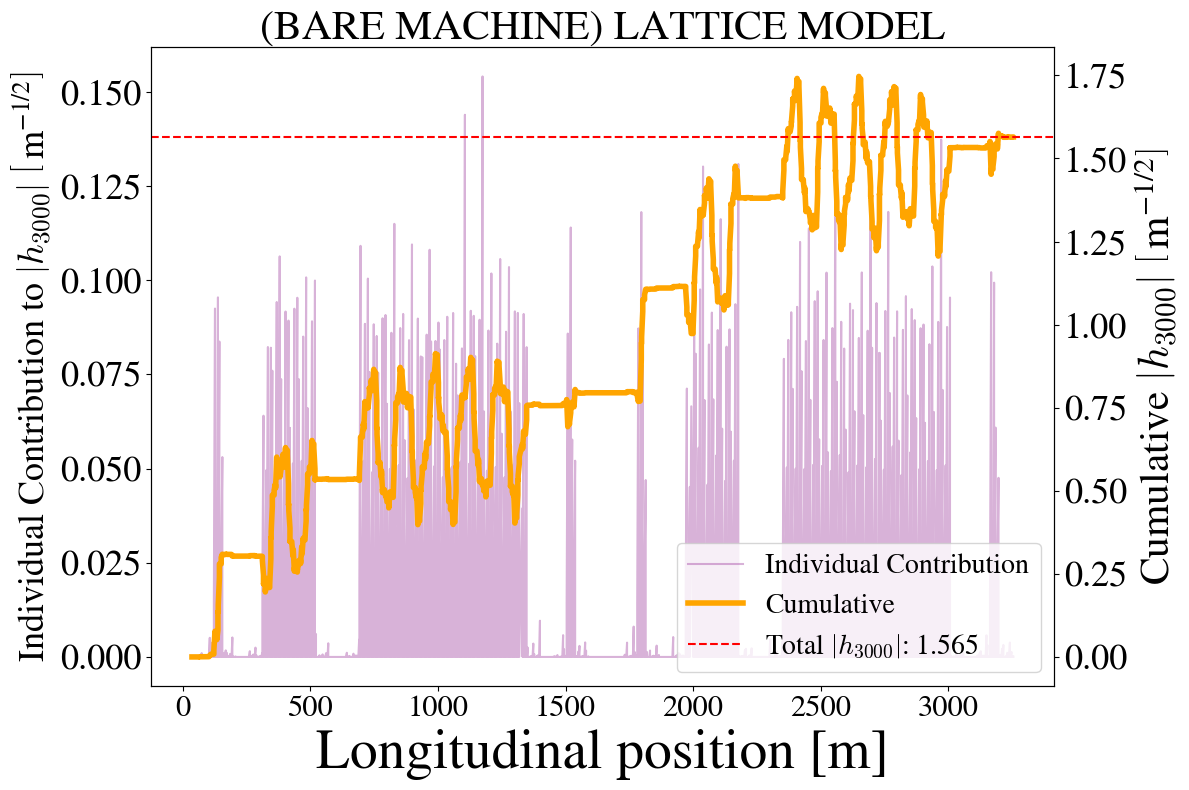
\includegraphics[width=\columnwidth]{chapter4/h3000_bare.png}
    \caption{Distribution of the $h_{3000}$ term around the ring with individual contributions from each relevant element and the cumulative sum from an arbitrary starting point.}
    \label{fig:h3000bare}
\end{figure}

\begin{figure}[H]
    \centering
    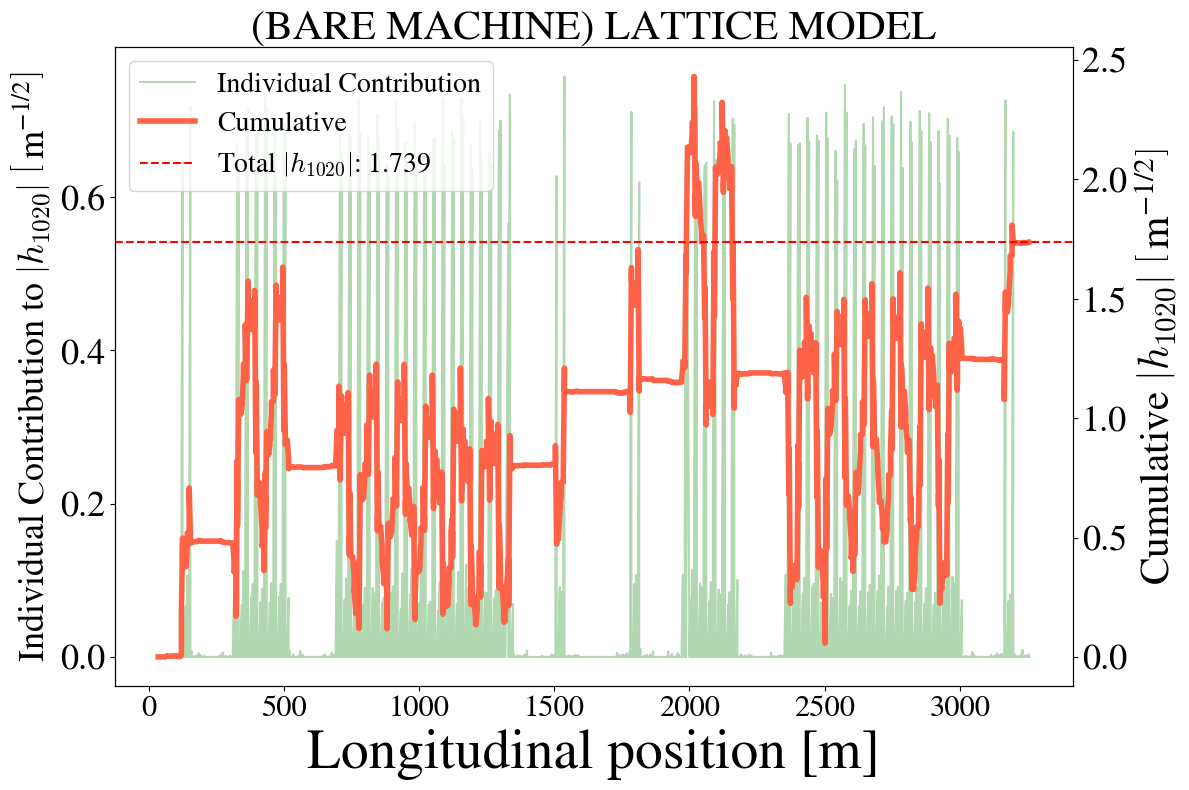
\includegraphics[width=\columnwidth]{chapter4/h1020_bare.png}
    \caption{Distribution of the $h_{1020}$ term around the ring with individual contributions from each relevant element and the cumulative sum from an arbitrary starting point.}
    \label{fig:h1020bare}
\end{figure}

\section{Measurement of Third Order RDTs}

\begin{equation}
    \label{eq:hxspect}
    h_x^{-}(N)= \hat{x} \pm \hat{p}_x = \sum_{jklm}HSL_{jklm}e^{2\pi i N \left[ \left( 1-j+k\right)Q_x+\left( m-l \right)Q_y\right]}
\end{equation}

\begin{equation}
    \label{eq:hyspect}
    h_y^{-}(N)= \hat{y} \pm \hat{p}_y = \sum_{jklm}VSL_{jklm}e^{2\pi i N \left[ \left( k-j\right)Q_x+\left(1-l+m \right)Q_y\right]}
\end{equation}

\begin{multline}
    \label{eq:hxpsi2}
    h_x^{-}(N)=\sqrt{2I_x}e^{i\left( \psi_x+\psi_{x_0}\right)} \\
    -2i \sum_{jklm} j f_{jklm} \left( 2I_x \right)^{\frac{j+k-1}{2}}\left( 2I_y \right)^{\frac{l+m}{2}}
    e^{i \left[ \left( 1-j+k\right)\left( \psi_x + \psi_{x_0} \right) +\left( m-l\right)\left( \psi_y + \psi_{y_0} \right)\right]}.
\end{multline}

\begin{multline}
    \label{eq:hypsi2}
    h_y^{-}(N)=\sqrt{2I_y}e^{i\left( \psi_y+\psi_{y_0}\right)} \\
    -2i \sum_{jklm} l f_{jklm} \left( 2I_x \right)^{\frac{j+k}{2}}\left( 2I_y \right)^{\frac{l+m-1}{2}}
    e^{i \left[ \left( k-j\right)\left( \psi_x + \psi_{x_0} \right) +\left( 1-l+m\right)\left( \psi_y + \psi_{y_0} \right)\right]}.
\end{multline}

\begin{figure}[H]
    \centering
    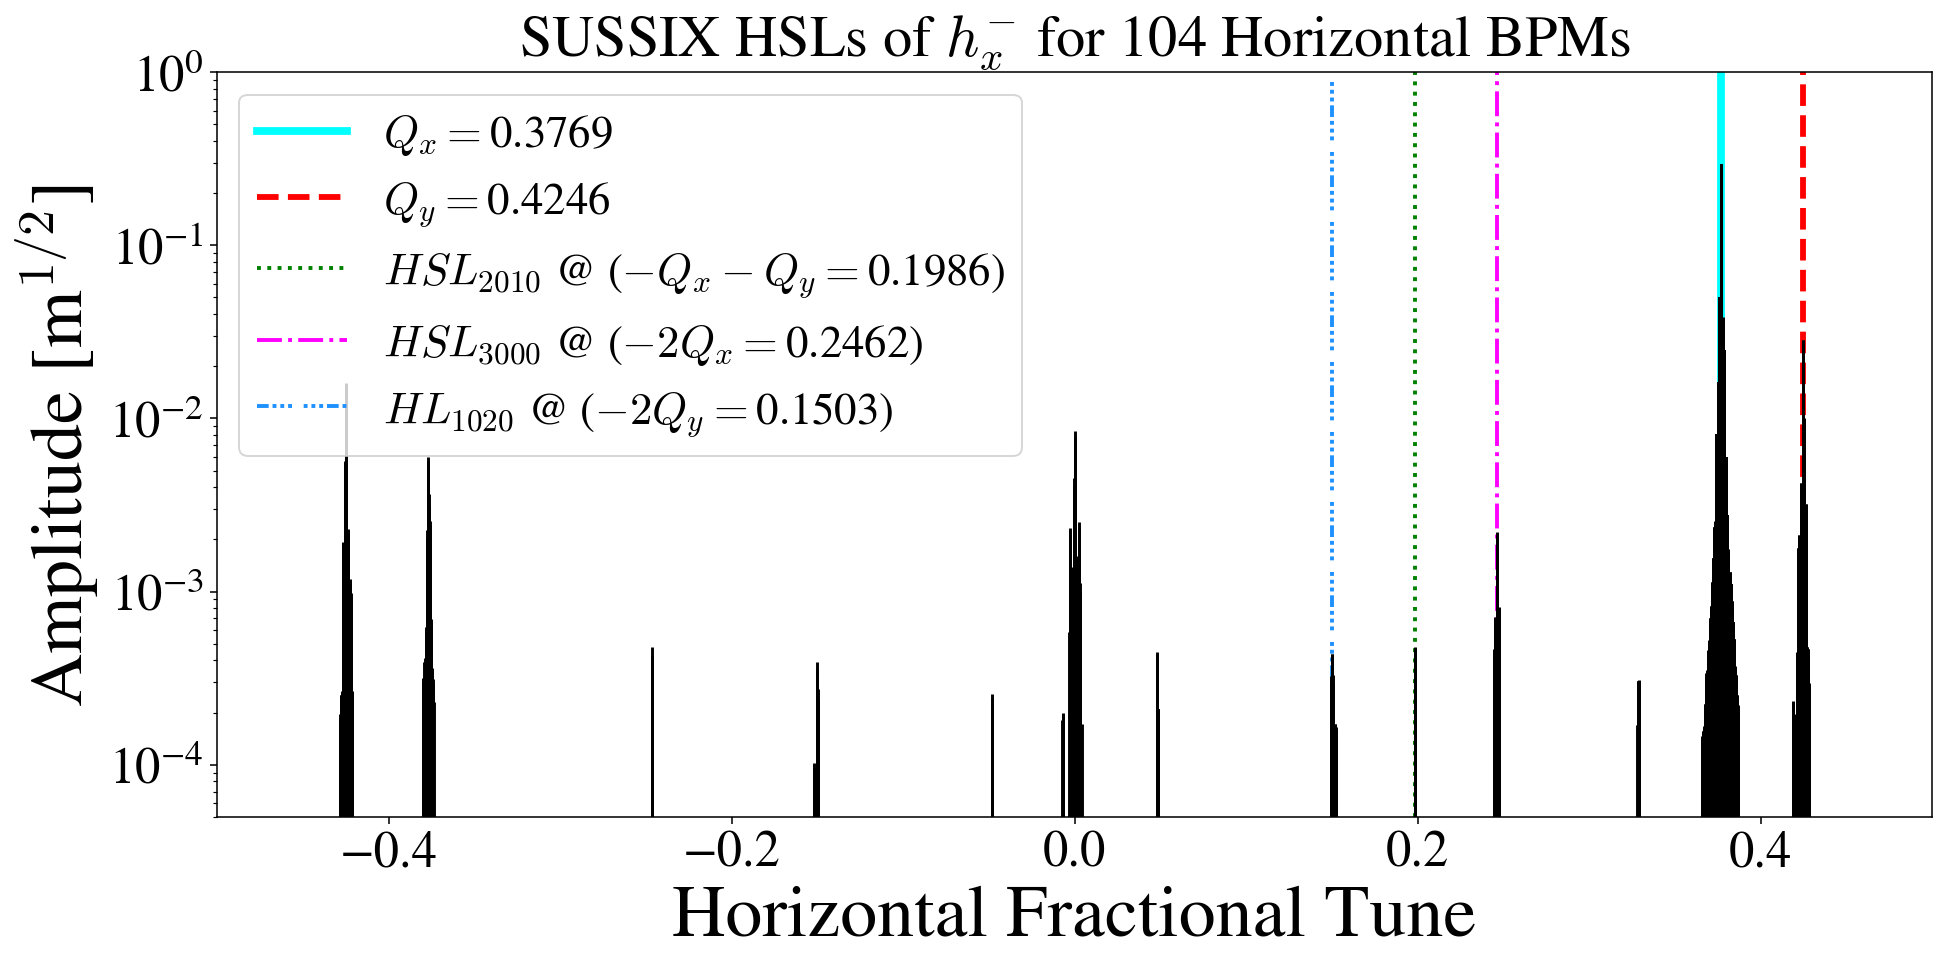
\includegraphics[width=\columnwidth]{chapter4/hxspect.png}
    \caption{Spectral lines of $h_x^{-}$ calculated with SUSSIX \cite{sussix}. The $h_x^{-}$ signal was reconstructed for the 104 Horizontal BPMs. The spectrum for all BPMs is superimposed in this plot.}
    \label{fig:hxspect1}
\end{figure}

\begin{figure}[H]
    \centering
    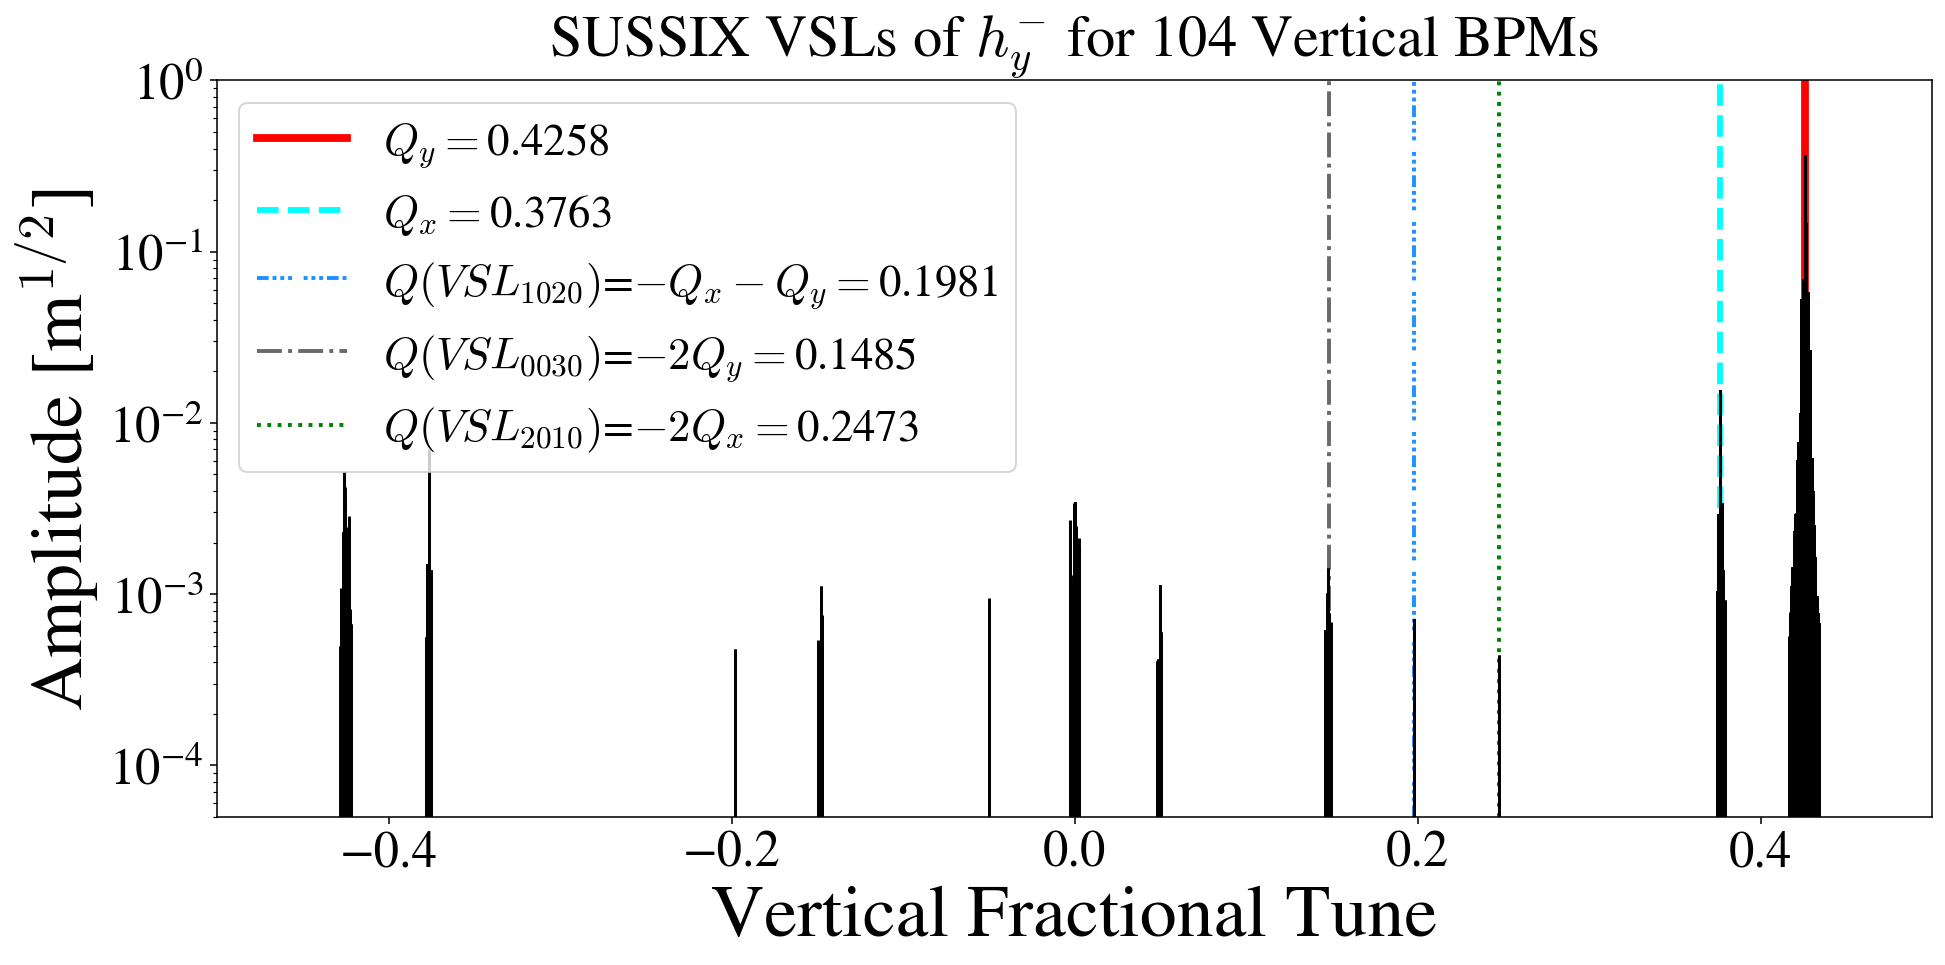
\includegraphics[width=\columnwidth]{chapter4/hyspect.png}
    \caption{Spectral lines of $h_y^{-}$ calculated with SUSSIX \cite{sussix}. The $h_y^{-}$ signal was reconstructed for the 104 Vertical BPMs. The spectrum for all BPMs is superimposed in this plot.}
    \label{fig:hyspect1}
\end{figure}

\begin{table}[H]
    \centering
    \caption{Corresponding RDTs and location of spectral lines for each resonance line.}
    \begin{tabular}{lcccc}
        \toprule
        \textbf{Resonance Line} & \textbf{Source} & \textbf{RDT} & \textbf{Hor. Spect.} & \textbf{Vert. Spect.} \\
        \midrule
            $3Q_x=76$     & Normal Sextupole    & $h_{3000}$           &  (-2,0)  & -       \\ %[3pt]
           $Q_x+2Q_y=74$   & Normal Sextupole    & $h_{1020}$            & (0,-2) & (-1,-1)       \\ %[3pt]
            $3Q_y=73$     & Skew Sextupole   & $h_{0030}$           & - & (0,-2)        \\ %[3pt]
            $2Q_x+Q_y=75$   & Skew Sextupole    & $h_{2010}$     & (-1,-1) & (-2,0)       \\
        \bottomrule
    \end{tabular}
    \label{tab:rdtlines}
\end{table}

\begin{figure}[H]
    \centering
    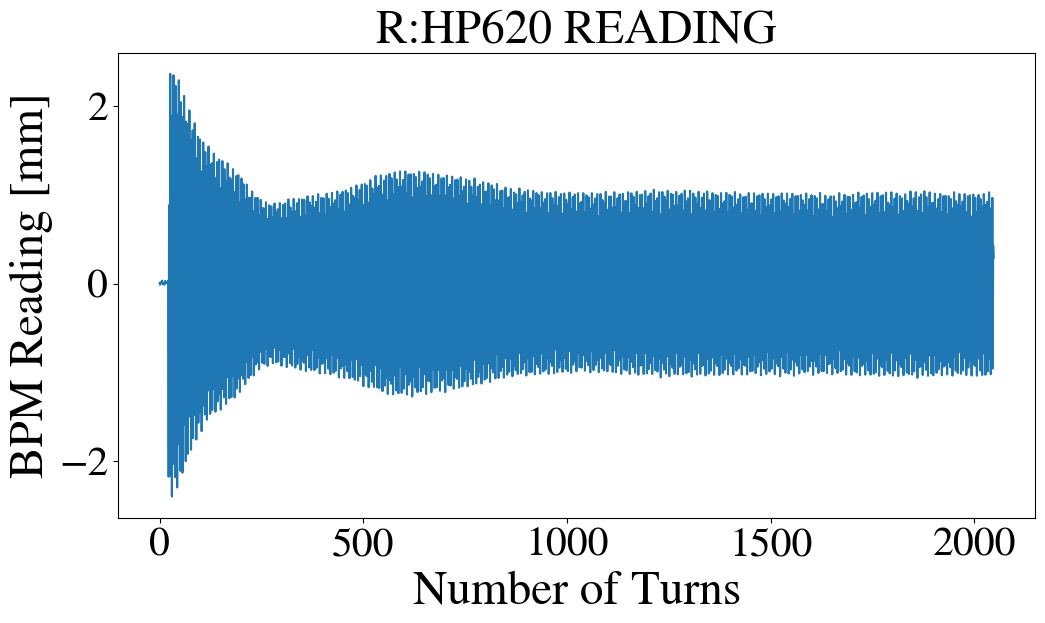
\includegraphics[width=\columnwidth]{chapter4/bpm_kick.png}
    \caption{}
    \label{fig:bpm_kick0}
\end{figure}

\begin{figure}[H]
    \centering
    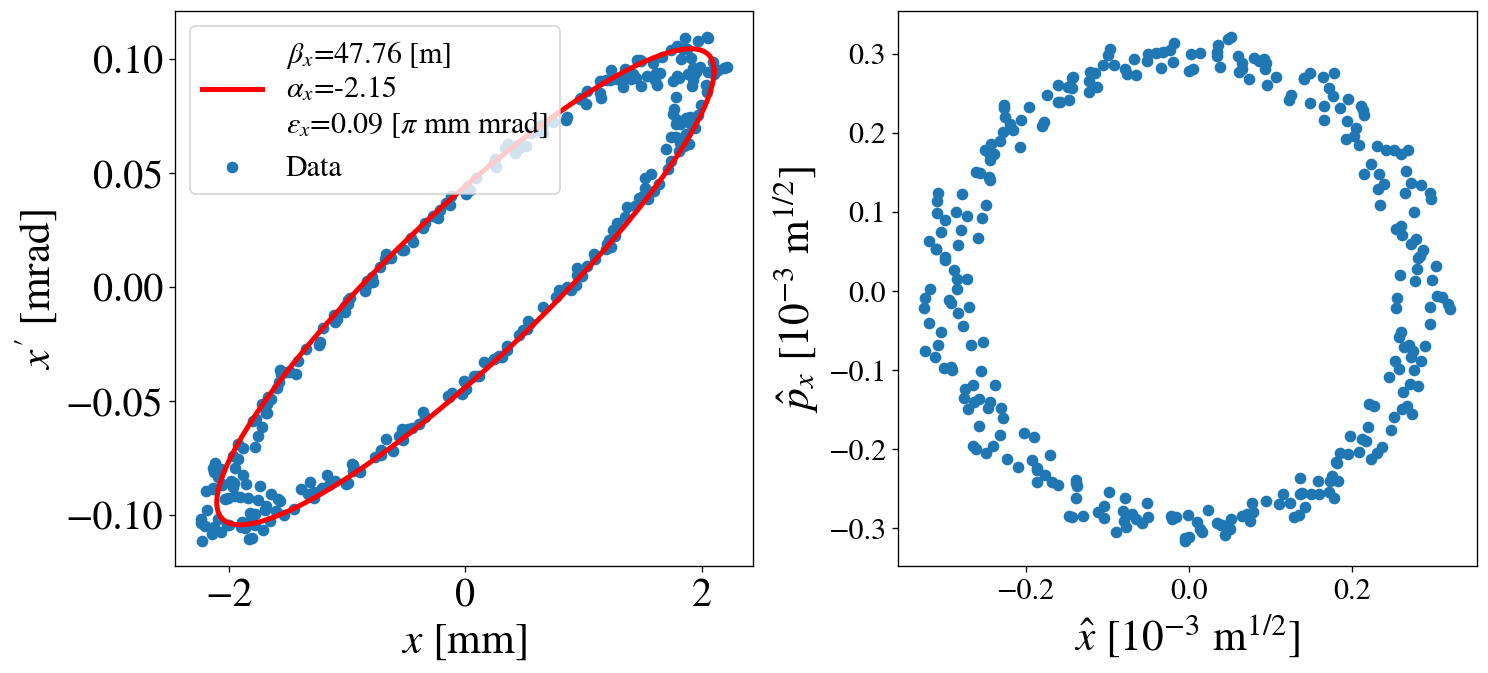
\includegraphics[width=\columnwidth]{chapter4/ellipse_data.png}
    \caption{}
    \label{fig:ellipse}
\end{figure}

\section{Compensation of RDTs}

For resonance compensation we have four dedicated normal sextupoles with currents that can be set to ($I_{sc220},I_{sc222},I_{sc319},I_{sc321}$) and four dedicated skew sextupoles with currents that can be set to ($I_{ss323},I_{ss323},I_{ss319},I_{ss321}$). As shown in the previous section one RDT can be cancelled out with the right kick from the correction elements, which means the resonances are corrected to first order. 

Nevertheless, by compensating one resonance line, other resonances  might become worse. This is why for simultaneous compensation, compensation currents will vary depending on the subsets of resonances to compensate. In principle, the currents $I_x$ needed in each correction element in order to cancel out the four bare machine RDTs, are given by the solution to this linear system of equations: 
\begin{equation}
    \begin{bmatrix}
        -|{h_{3000}}|  \cos (\psi_{3000})\\
        -|{h_{3000}}|  \sin (\psi_{3000})\\
        -|{h_{1020}}|  \cos (\psi_{1020})\\
        -|{h_{1020}}|  \sin (\psi_{1020})\\
        -|{h_{0030}}|  \cos (\psi_{3000})\\
        -|{h_{0030}}|  \sin (\psi_{3000})\\
        -|{h_{2010}}|  \cos (\psi_{1020})\\
        -|{h_{2010}}|  \sin (\psi_{1020})\\
      \end{bmatrix}_{(Bare)}
    =
      \boldsymbol{M}
    \begin{bmatrix}
        I_{sc220} \\
        I_{sc222} \\
        I_{sc319} \\
        I_{sc321} \\
        I_{ss223} \\
        I_{ss323} \\
        I_{ss319} \\
        I_{ss321} \\
      \end{bmatrix}
    \label{eq:system}
\end{equation}
where $M_{ij}$ is the response matrix for the RDTs with respect to the currents, and includes any roll that can happen for the correction sextupoles. This response matrix $M_{ij}$ can be calculated by scanning the currents in each correction element and looking at the response from the real and imaginary part of the RDTs, i.e., $h_{jklm}=|h_{jklm}|e^{i\psi_{jklm}}$. 

In reality, there are limitations to solving equation \ref{eq:system}. The first one is that all the RDTs ($h_{jklm}$) may not be accessible for measurement, given that they may not show up as a spectral line.  Another limitation is that the solution for the currents may be outside the maximum limits for the correction elements. 

One can also try to cancel out a subset of RDTs from equation \ref{eq:system}, including only one RDT. For example, in order to compensate $3 Q_x=76$, the system of equations to be solved is:

\begin{equation}
    \begin{bmatrix}
        -|{h_{3000}}|  \cos (\psi_{3000})\\
        -|{h_{3000}}|  \sin (\psi_{3000})\\
        0\\
        0\\
      \end{bmatrix}_{(Bare)}
    =
    \begin{bmatrix}
        M_{11} & M_{12} & M_{13} & M_{14} \\
        M_{21} & M_{22} & M_{23} & M_{24} \\
        1 & 1 & 0 & 0 \\
        0 & 0 & 1 & 1 \\
    \end{bmatrix}
    \begin{bmatrix}
        I_{sc220} \\
        I_{sc222} \\
        I_{sc319} \\
        I_{sc321} \\
      \end{bmatrix}
    \label{eq:system1}
\end{equation}

\begin{figure}[H]
    \centering
    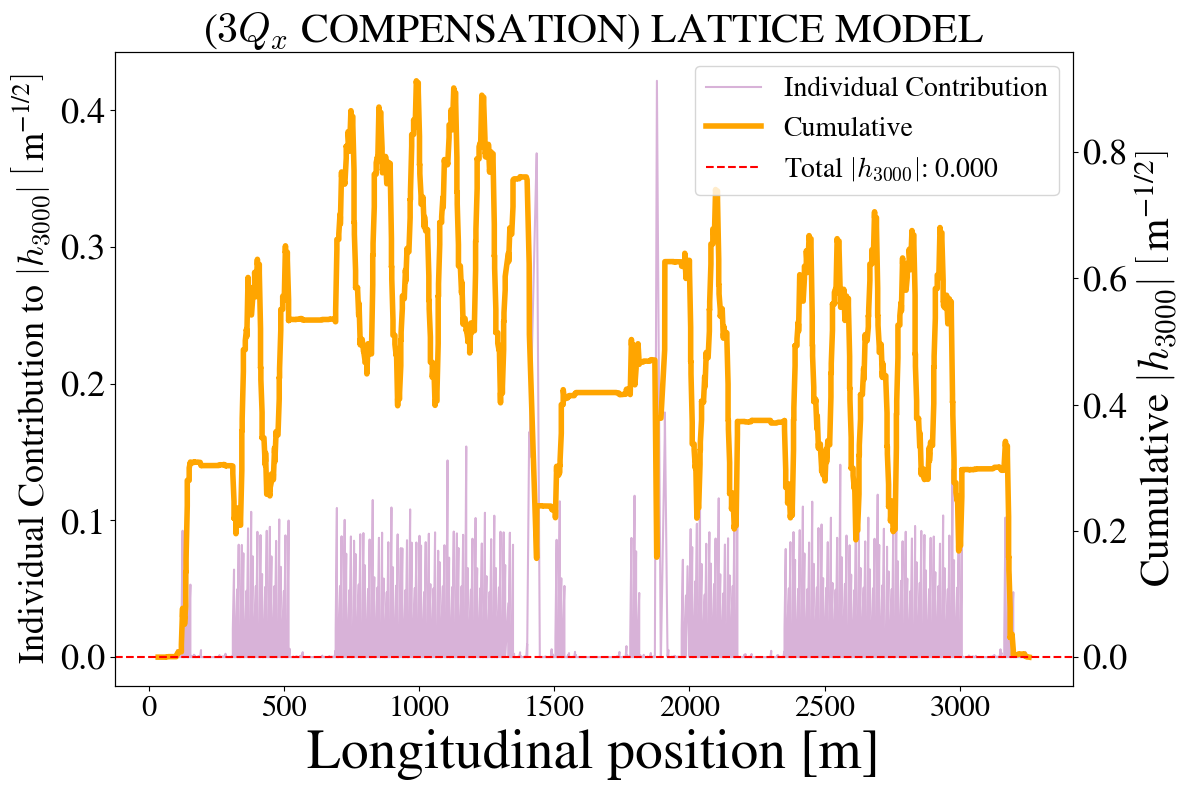
\includegraphics[width=\columnwidth]{chapter4/h3000_3qxcomp.png}
    \caption{Distribution of the $h_{3000}$ term around the ring with individual contributions from each relevant element and the cumulative sum from an arbitrary starting point when correction elements are set to compensate $3Q_x=76$, i.e., $h_{3000}=0$.}
    \label{fig:h3000_3qxcomp}
\end{figure}

\begin{figure}[H]
    \centering
    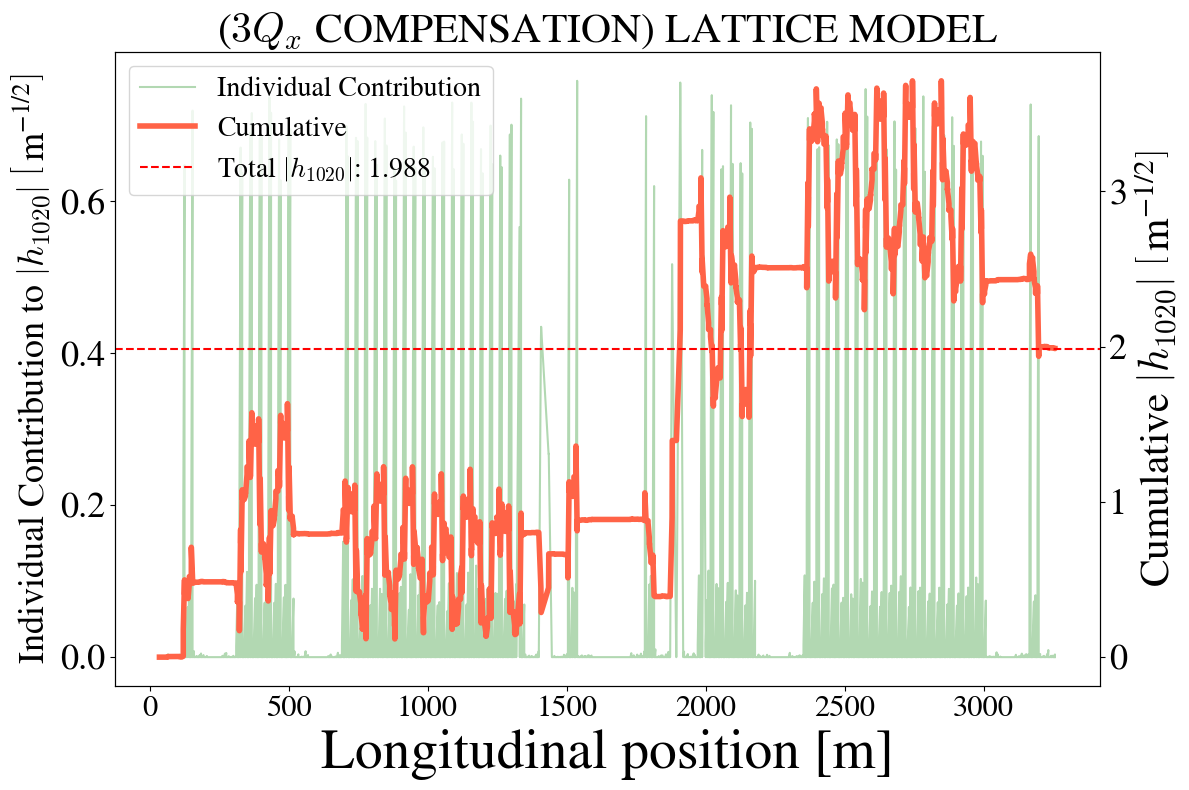
\includegraphics[width=\columnwidth]{chapter4/h1020_3qxcomp.png}
    \caption{Distribution of the $h_{1020}$ term around the ring with individual contributions from each relevant element and the cumulative sum from an arbitrary starting point when correction elements are set to compensate $3Q_x=76$, i.e., $h_{3000}=0$.}
    \label{fig:h1020_3qxcomp}
\end{figure}

\section{Optimization of Compensation Currents}

\section{Experimental Verification of Compensation}

\subsection{\label{sec:lossmaps}Dynamic Loss Maps}

One effective method for visualizing resonance compensation involves constructing dynamic loss maps. To generate these representations, specialized quadrupoles responsible for controlling the tune of the Recycler are gradually adjusted to map out the desired tune area. Throughout this process, the beam loss rate is meticulously measured and interpolated across the specified region. This is done in the horizontal and vertical direction. The initial horizontal scan is generated by maintaining a constant vertical tune while implementing a horizontal tune ramp ranging from $Q_x=25.47$ to $Q_x=25.31$. Subsequently, the vertical tune, initially set as \textit{constant} at $Q_y=24.47$, is adjusted incrementally to $Q_y=24.31$ in steps of 0.005, with intensity data recorded at each step. Conversely, for the vertical scan, the roles are reversed: the horizontal tune remains constant while a vertical tune ramp progresses from $Q_y=24.47$ to $Q_y=24.31$. Then, the \textit{constant} horizontal tune is varied from $Q_x=25.47$ to $Q_y=25.31$ in steps of 0.005. The resulting intensity data from both scans can be differentiated, normalized by the instantaneous intensity, and interpolated within a two-dimensional grid to construct plots akin to those depicted in Figs. \ref{fig:bare_nocomments} and \ref{fig:bare_comments}. Figure \ref{fig:bare_nocomments} demonstrates the initial machine scan without any compensation. If plotted alongside the theoretical positions of the lines as in Fig. \ref{fig:bare_comments}, the beam loss bands align with the resonance lines. 

Figure \ref{fig:bare_comments} illustrates the correspondence between the loss patterns and the theoretical positions of resonance lines. A slight deviation exists between the set tune and the actual tune due to calibration adjustments from the tune trombone program. However, despite this variance, the resonance line configuration within the loss pattern facilitates the visualization of each resonance's strength. Specifically, a higher normalized loss at a particular tune location indicates a stronger Resonance Driving Term (RDT) for the corresponding resonance line. Within Figs. \ref{fig:bare_nocomments} and \ref{fig:bare_comments}, third, fourth, and even traces of fifth-order resonance lines are discernible, with third-order resonance lines exhibiting the greatest prominence.

Figure \ref{fig:lossmaps} depicts dynamic loss maps representing various configurations of the compensation sextupoles. Specifically, Fig. \ref{fig:sfig1} illustrates the loss map for the bare machine, where no compensation sextupoles are activated, while Fig. \ref{fig:sfig2} and Fig. \ref{fig:sfig3} demonstrate compensation for a single resonance line each. In the case of $3Q_x$ compensation, the four normal sextupoles are adjusted to the calculated compensation currents using the RDT response matrix method. Moreover, a comparison between Fig. \ref{fig:sfig2} and Fig. \ref{fig:sfig1} clearly indicates a reduction of normalized losses by two orders of magnitude at the $3Q_x$ line with compensation. This observation holds true for the $3Q_y$ compensation as well, as shown in Fig. \ref{fig:sfig3}.

Figures \ref{fig:sfig4}, \ref{fig:sfig5}, and \ref{fig:sfig6} showcase the optimal configurations of compensation sextupoles designed to address multiple resonance lines simultaneously. It's important to note that while attempting to compensate for one or multiple resonance lines, there's a possibility that other resonance lines may strengthen. This is evident in the explicit case depicted in Fig. \ref{fig:sfig6}, where compensating for $3Q_y$ and $Q_x+2Q_y$ leads to the amplification of the $2Q_x+Q_y$ resonance. Such occurrences pose a limitation when aiming to compensate for more than two resonance lines, as the compensation currents tend to increase. There exists a constraint on the currents supplied to the compensation sextupoles. For instance, in compensating both normal sextupole lines, $3Q_x$ and $Q_x+2Q_y$, the required currents exceed the current limit. Ongoing efforts are focused on reducing the compensation currents in this specific scenario. Section \ref{sec:addsexts} summarizes some of these efforts, where additional sextupoles have been installed in order to decrease the currents that cancel out both the $h_{3000}$ and $h_{1020}$ RDTs.

Another notable detail evident in Figs. \ref{fig:sfig1}-\ref{fig:sfig6} is the presence of white areas within the loss maps, indicating regions where there was insufficient beam to accurately map out the losses. In certain configurations of the compensation sextupoles, the combined weakening of the third-order resonance lines occurs in a manner that leaves some beam remaining beyond these lines. It could be argued that conducting two additional scans, injecting from the left and bottom, could effectively map out these inaccessible regions. Such an enhancement could be considered as a future upgrade to these dynamic loss maps. Ultimately, all the plots presented in Fig. \ref{fig:lossmaps} demonstrate various potential configurations that open up regions of tune space for utilization during operations, enabling the accommodation of high-intensity beams.

\begin{figure}[H]
    \centering
    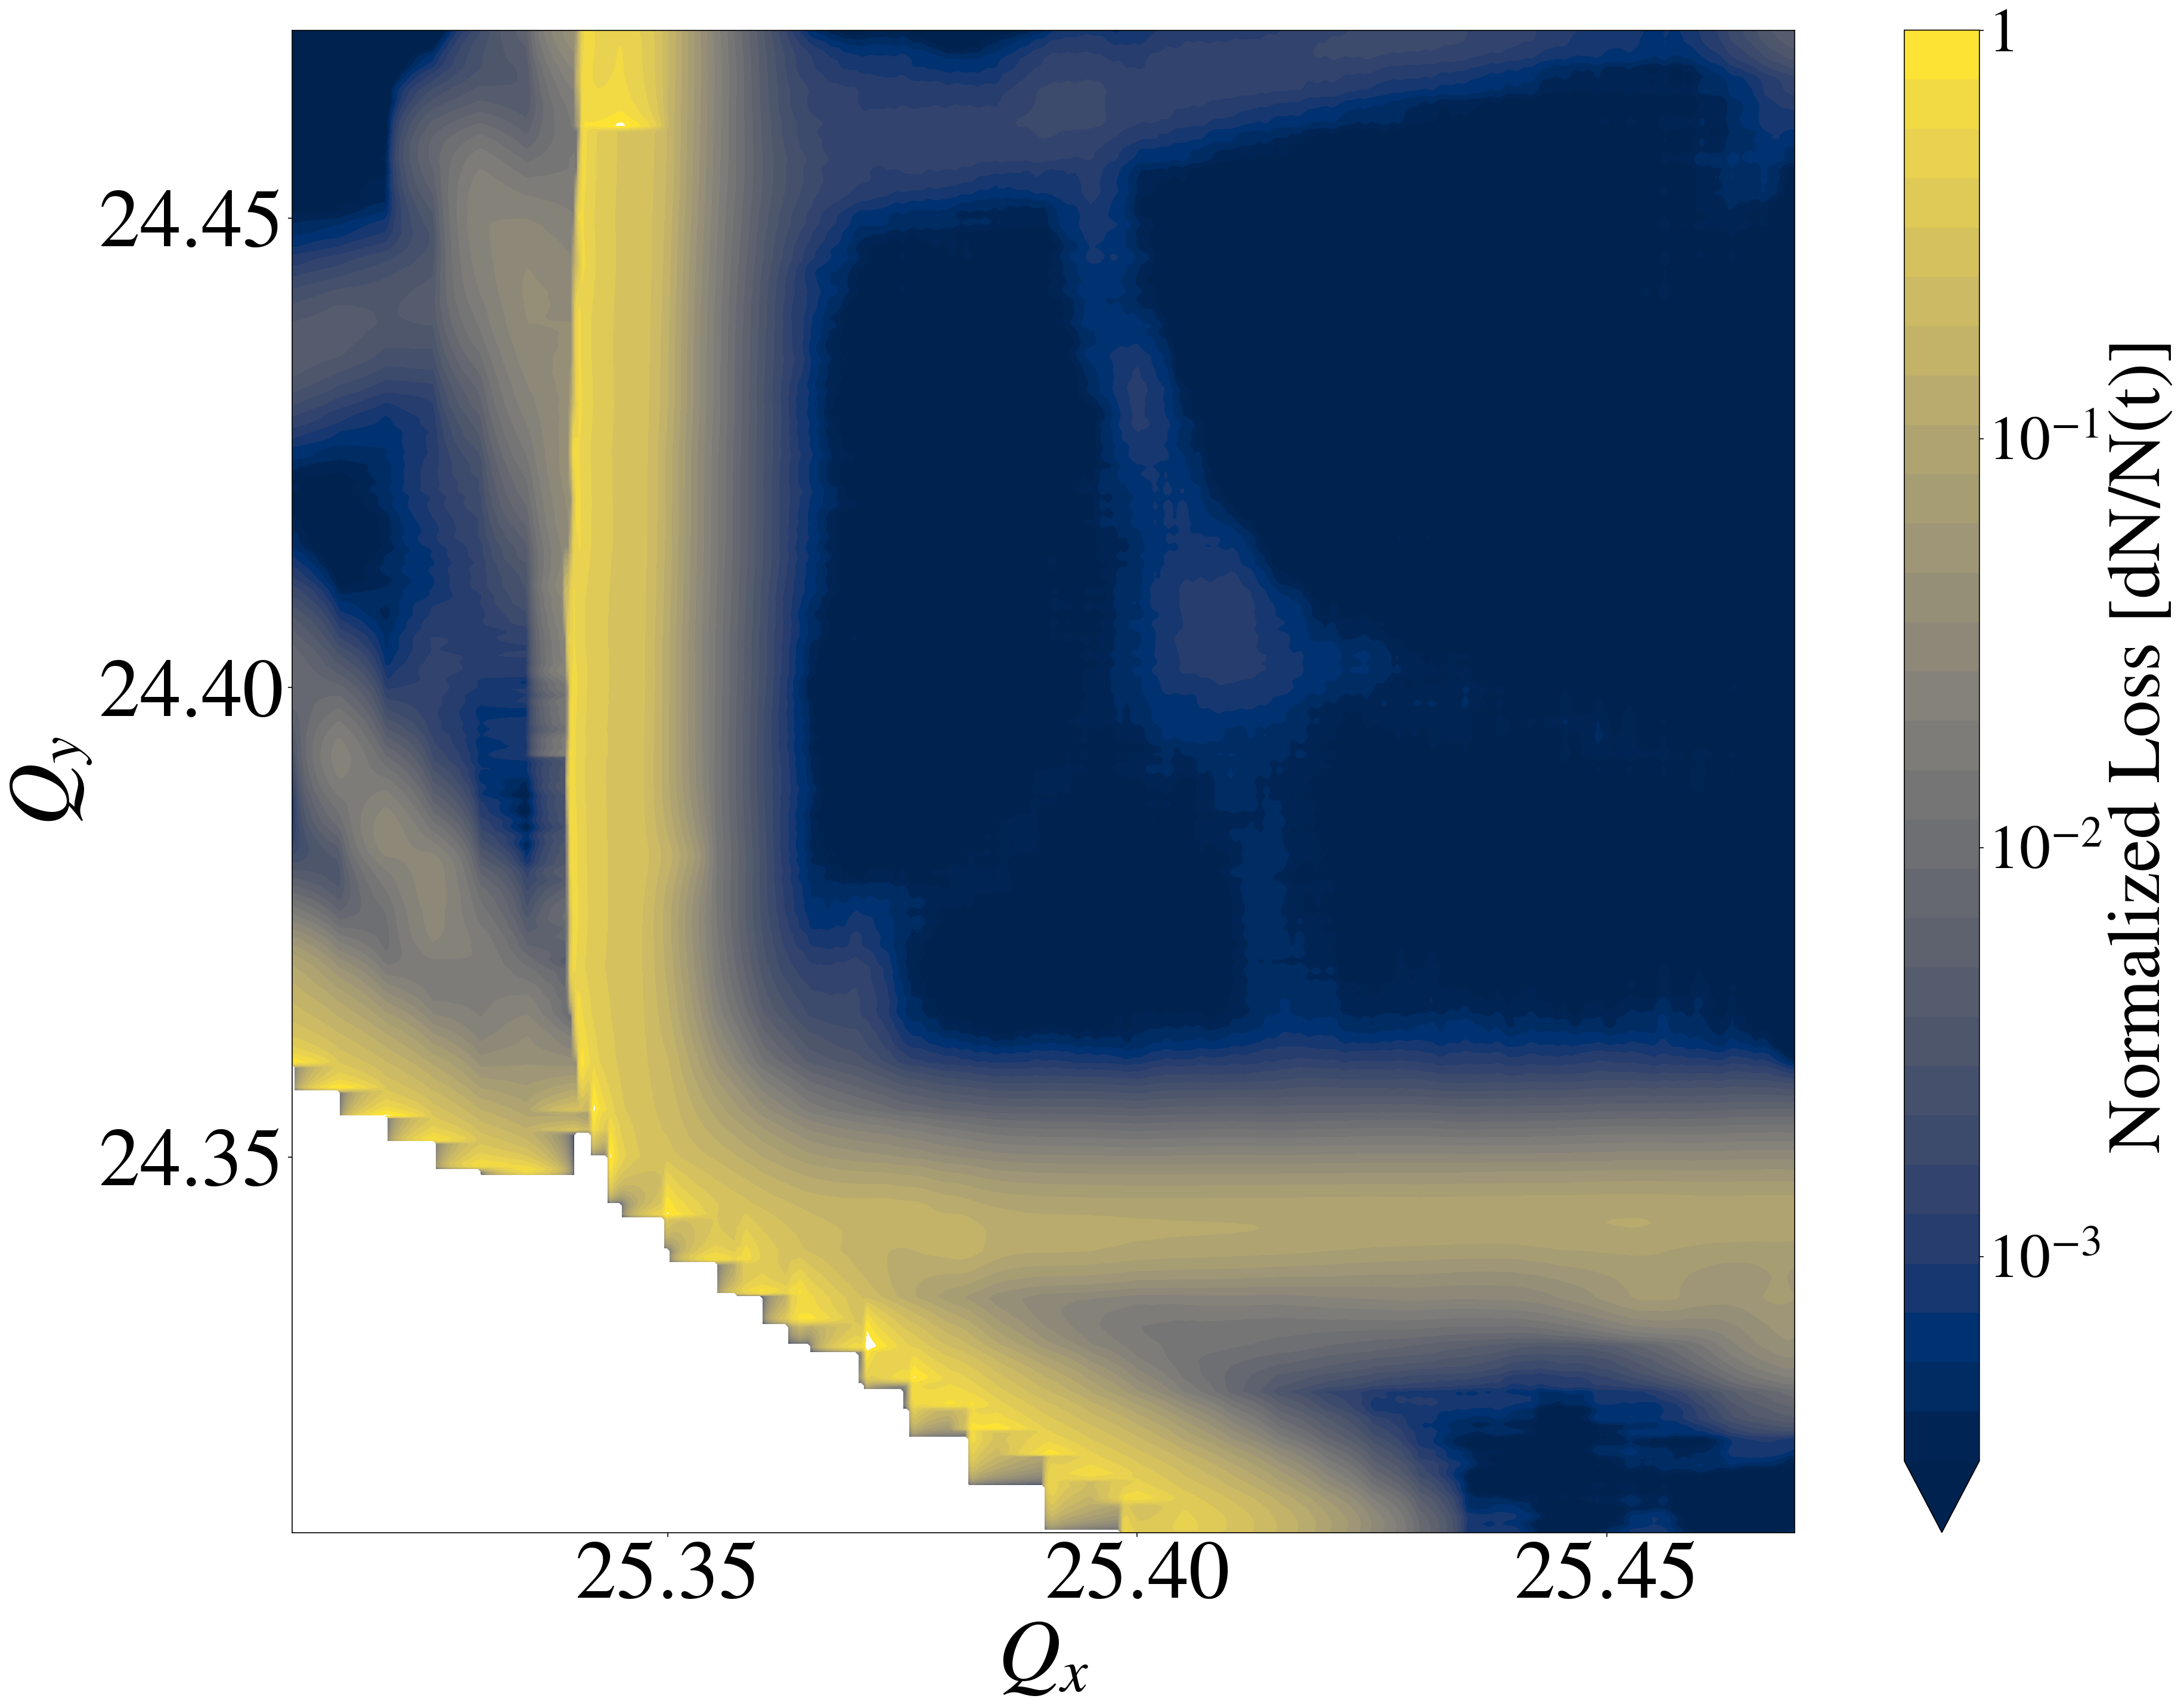
\includegraphics[width=\columnwidth]{chapter4/bare.png}
    \caption{Dynamic loss map from ramping the tunes with an interval of $\Delta Q_u=0.005$ in both directions. The directions of scan are from left to right and top to bottom. The results are superimposed in this plot.}
    \label{fig:bare_nocomments}
\end{figure}

\begin{figure}[H]
    \centering
    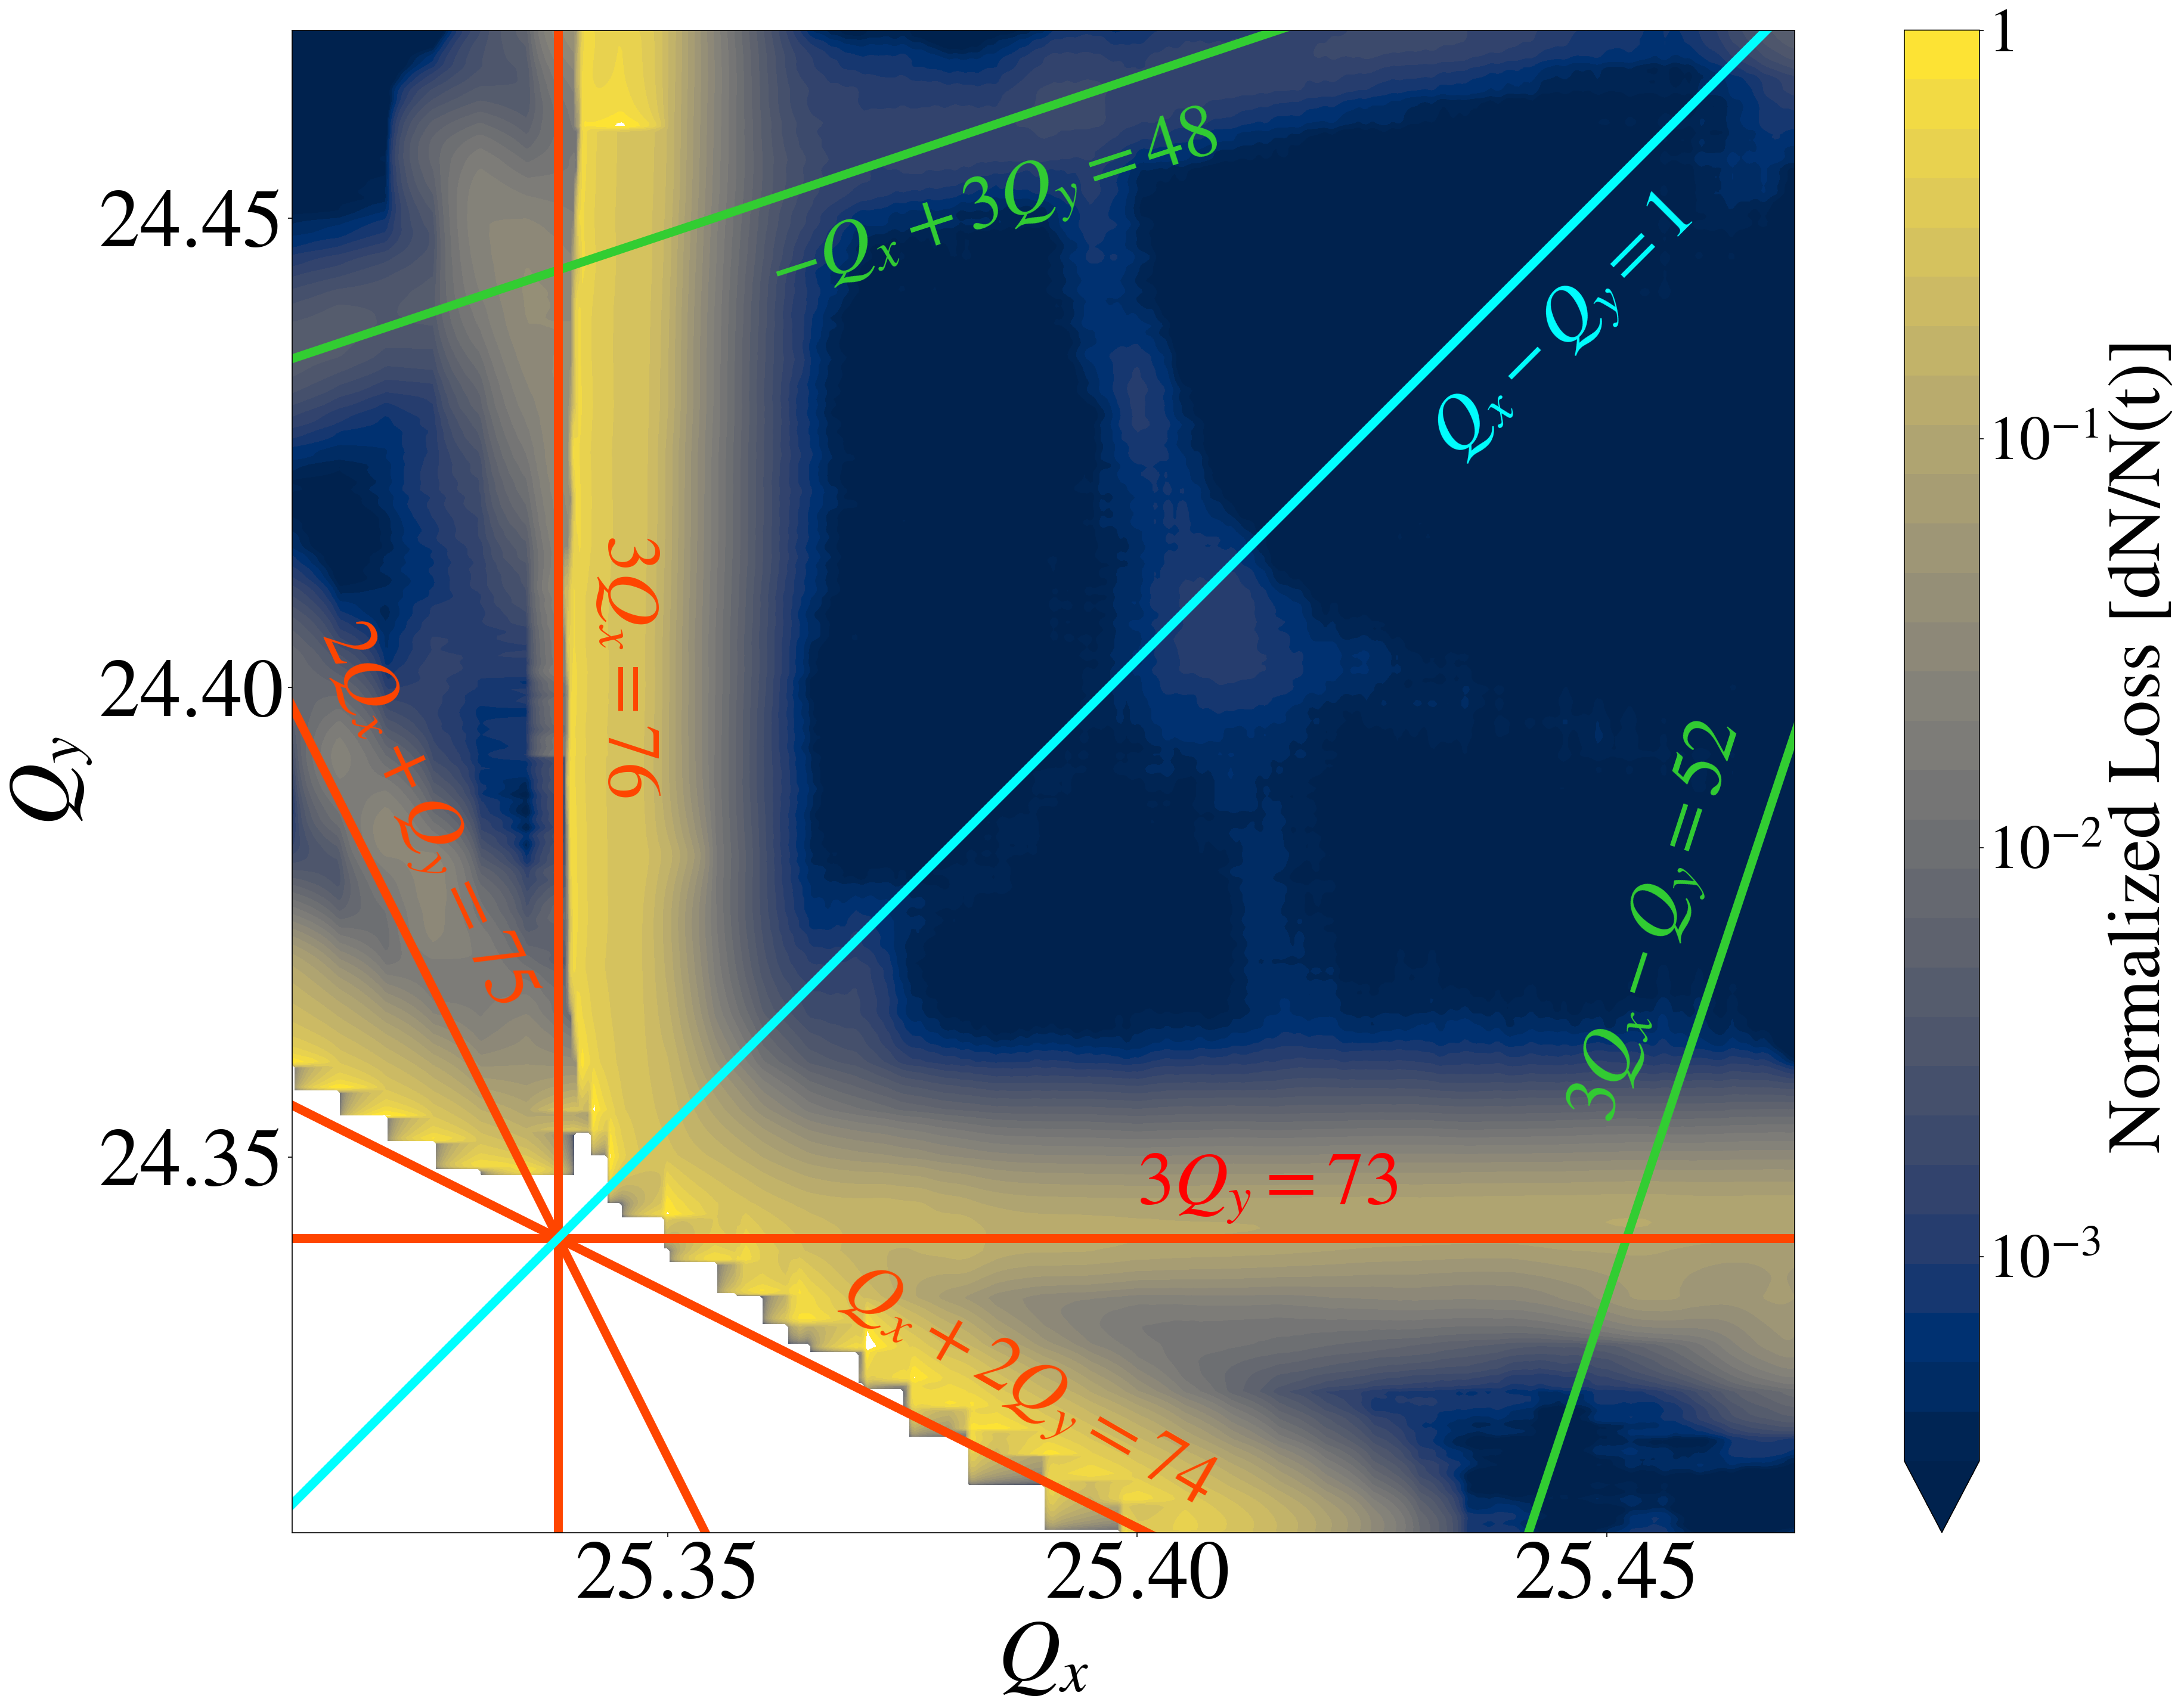
\includegraphics[width=\columnwidth]{chapter4/bare_comments.png}
    \caption{Dynamic loss map with the corresponding lines from Fig. \ref{fig:rrtd} drawn on top.}
    \label{fig:bare_comments}
\end{figure}


\newpage
\begin{figure}[H]

    \centering
    \begin{subfigure}{.49\textwidth}
      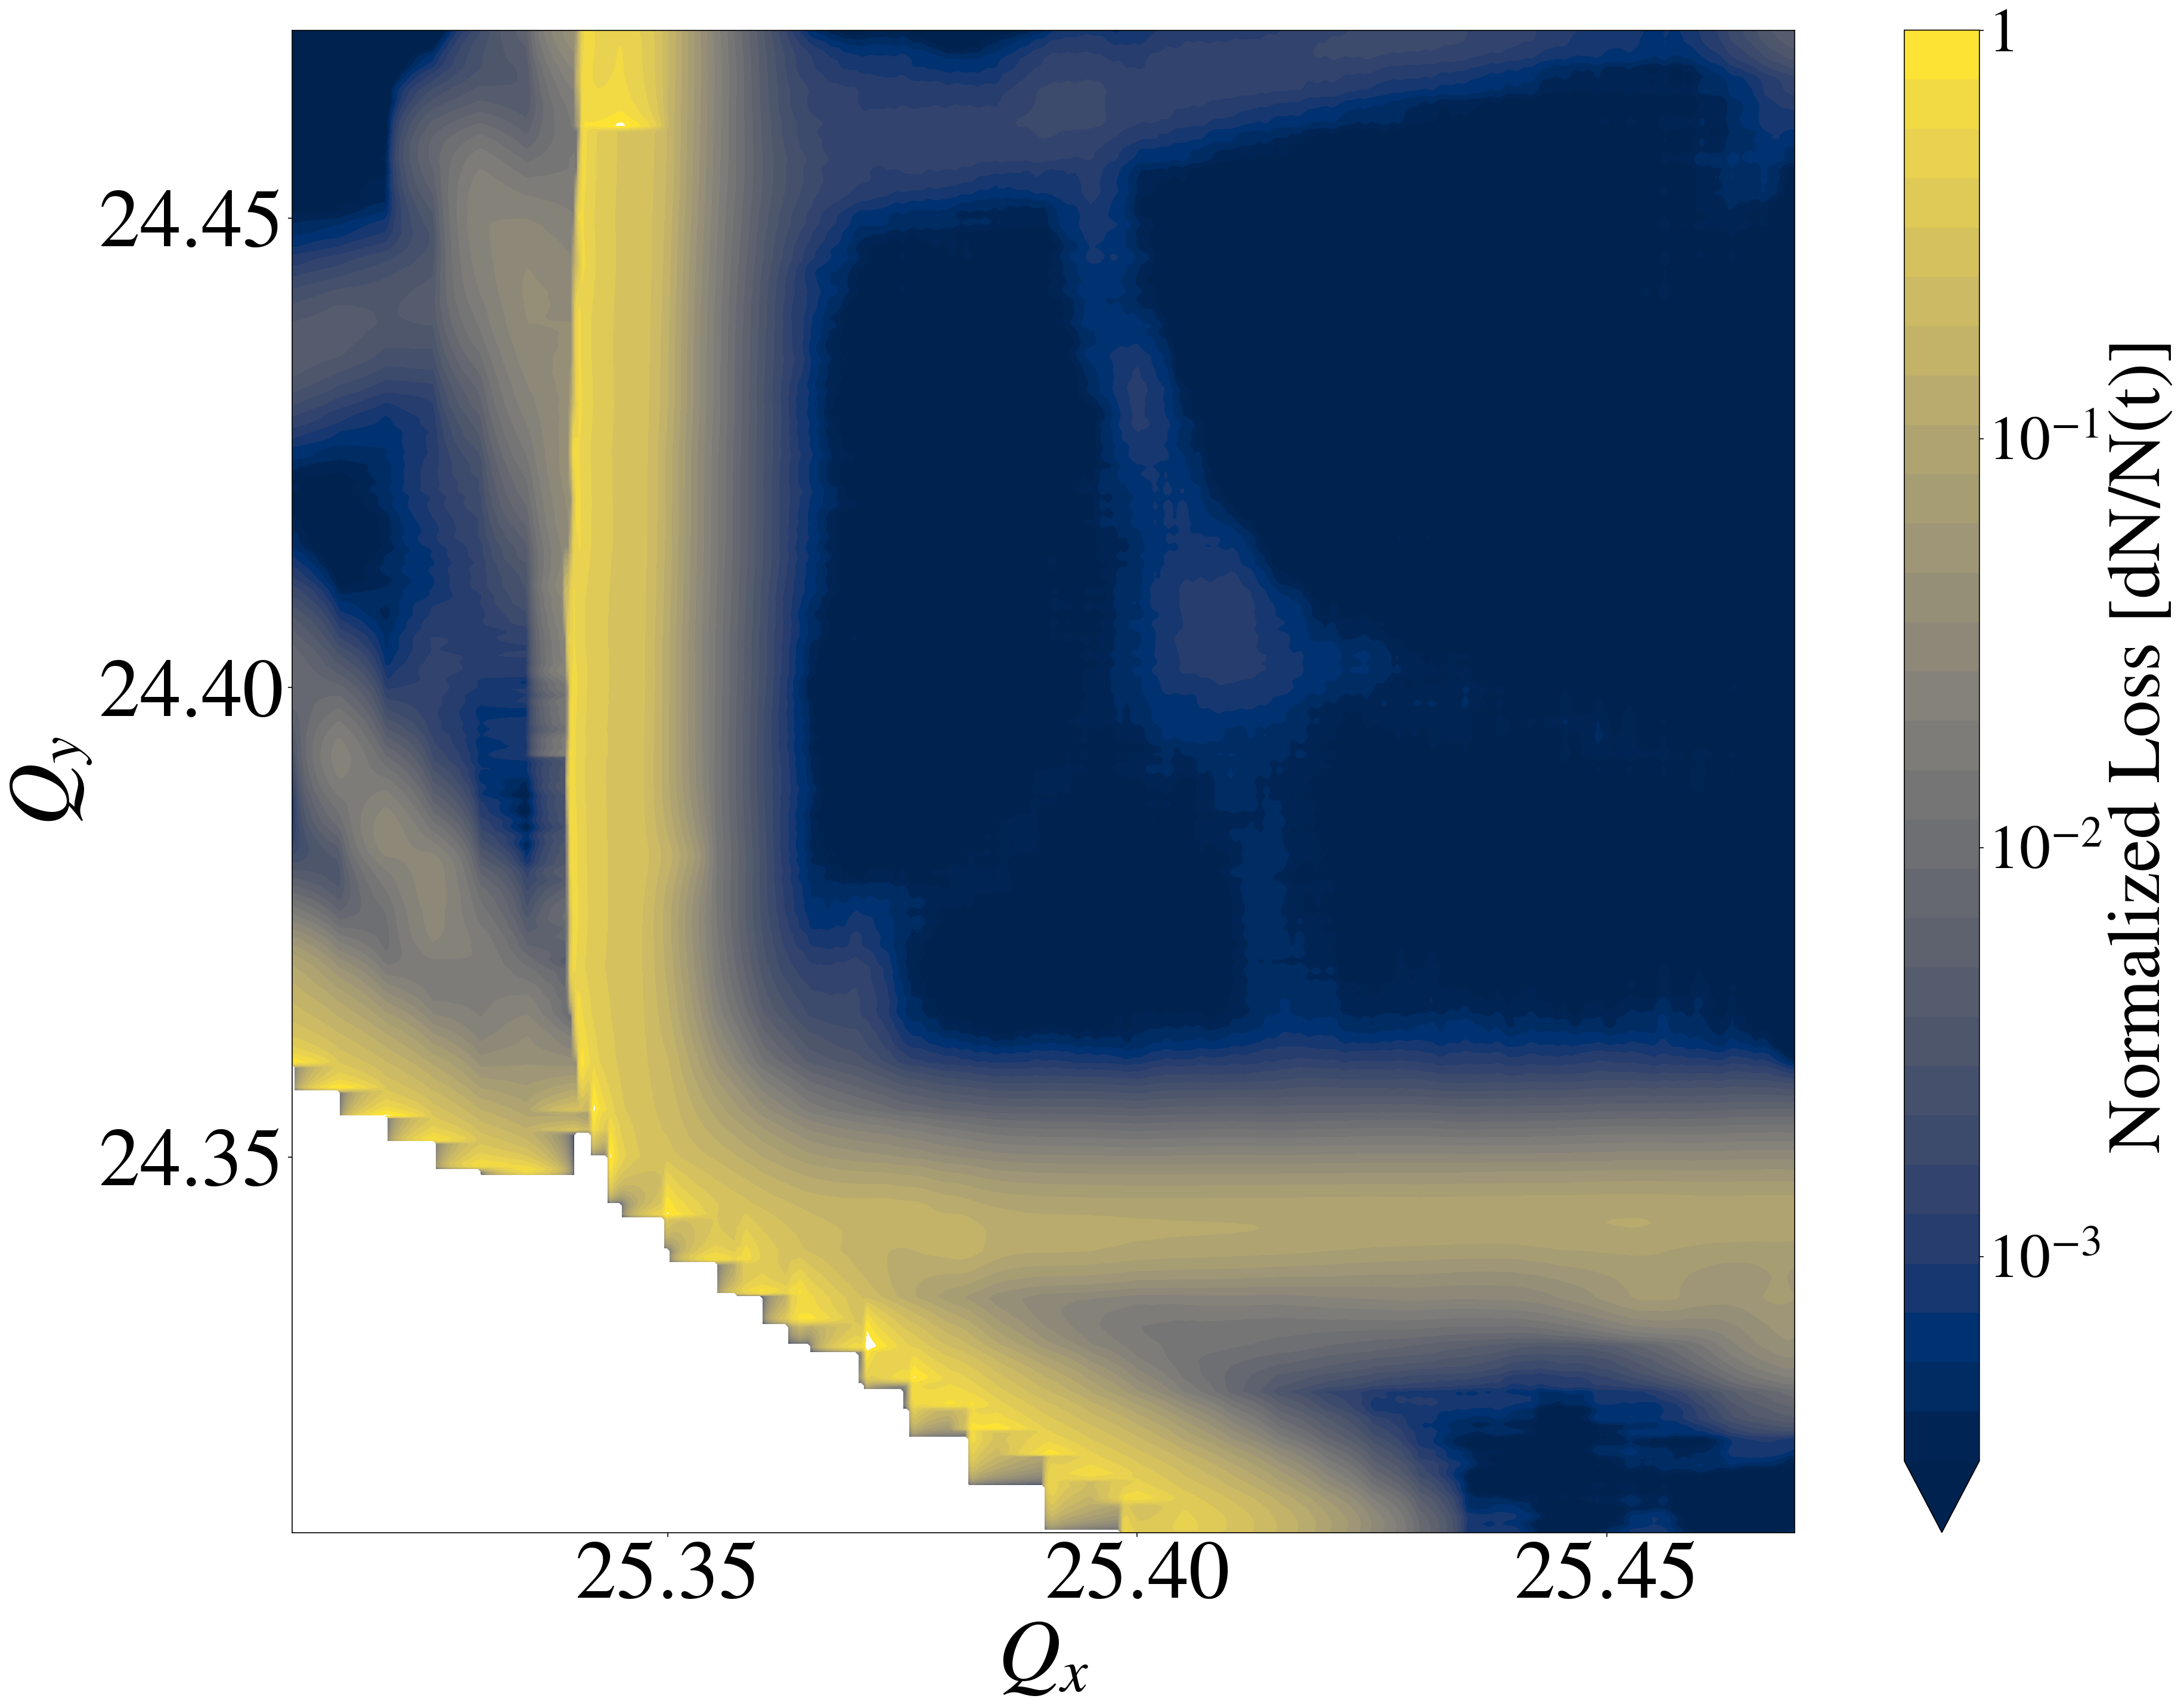
\includegraphics[width=0.98\linewidth]{chapter4/bare.png}
      \caption{Bare machine}
      \label{fig:sfig1}
    \end{subfigure}%
    \hfill
    \begin{subfigure}{.49\textwidth}
      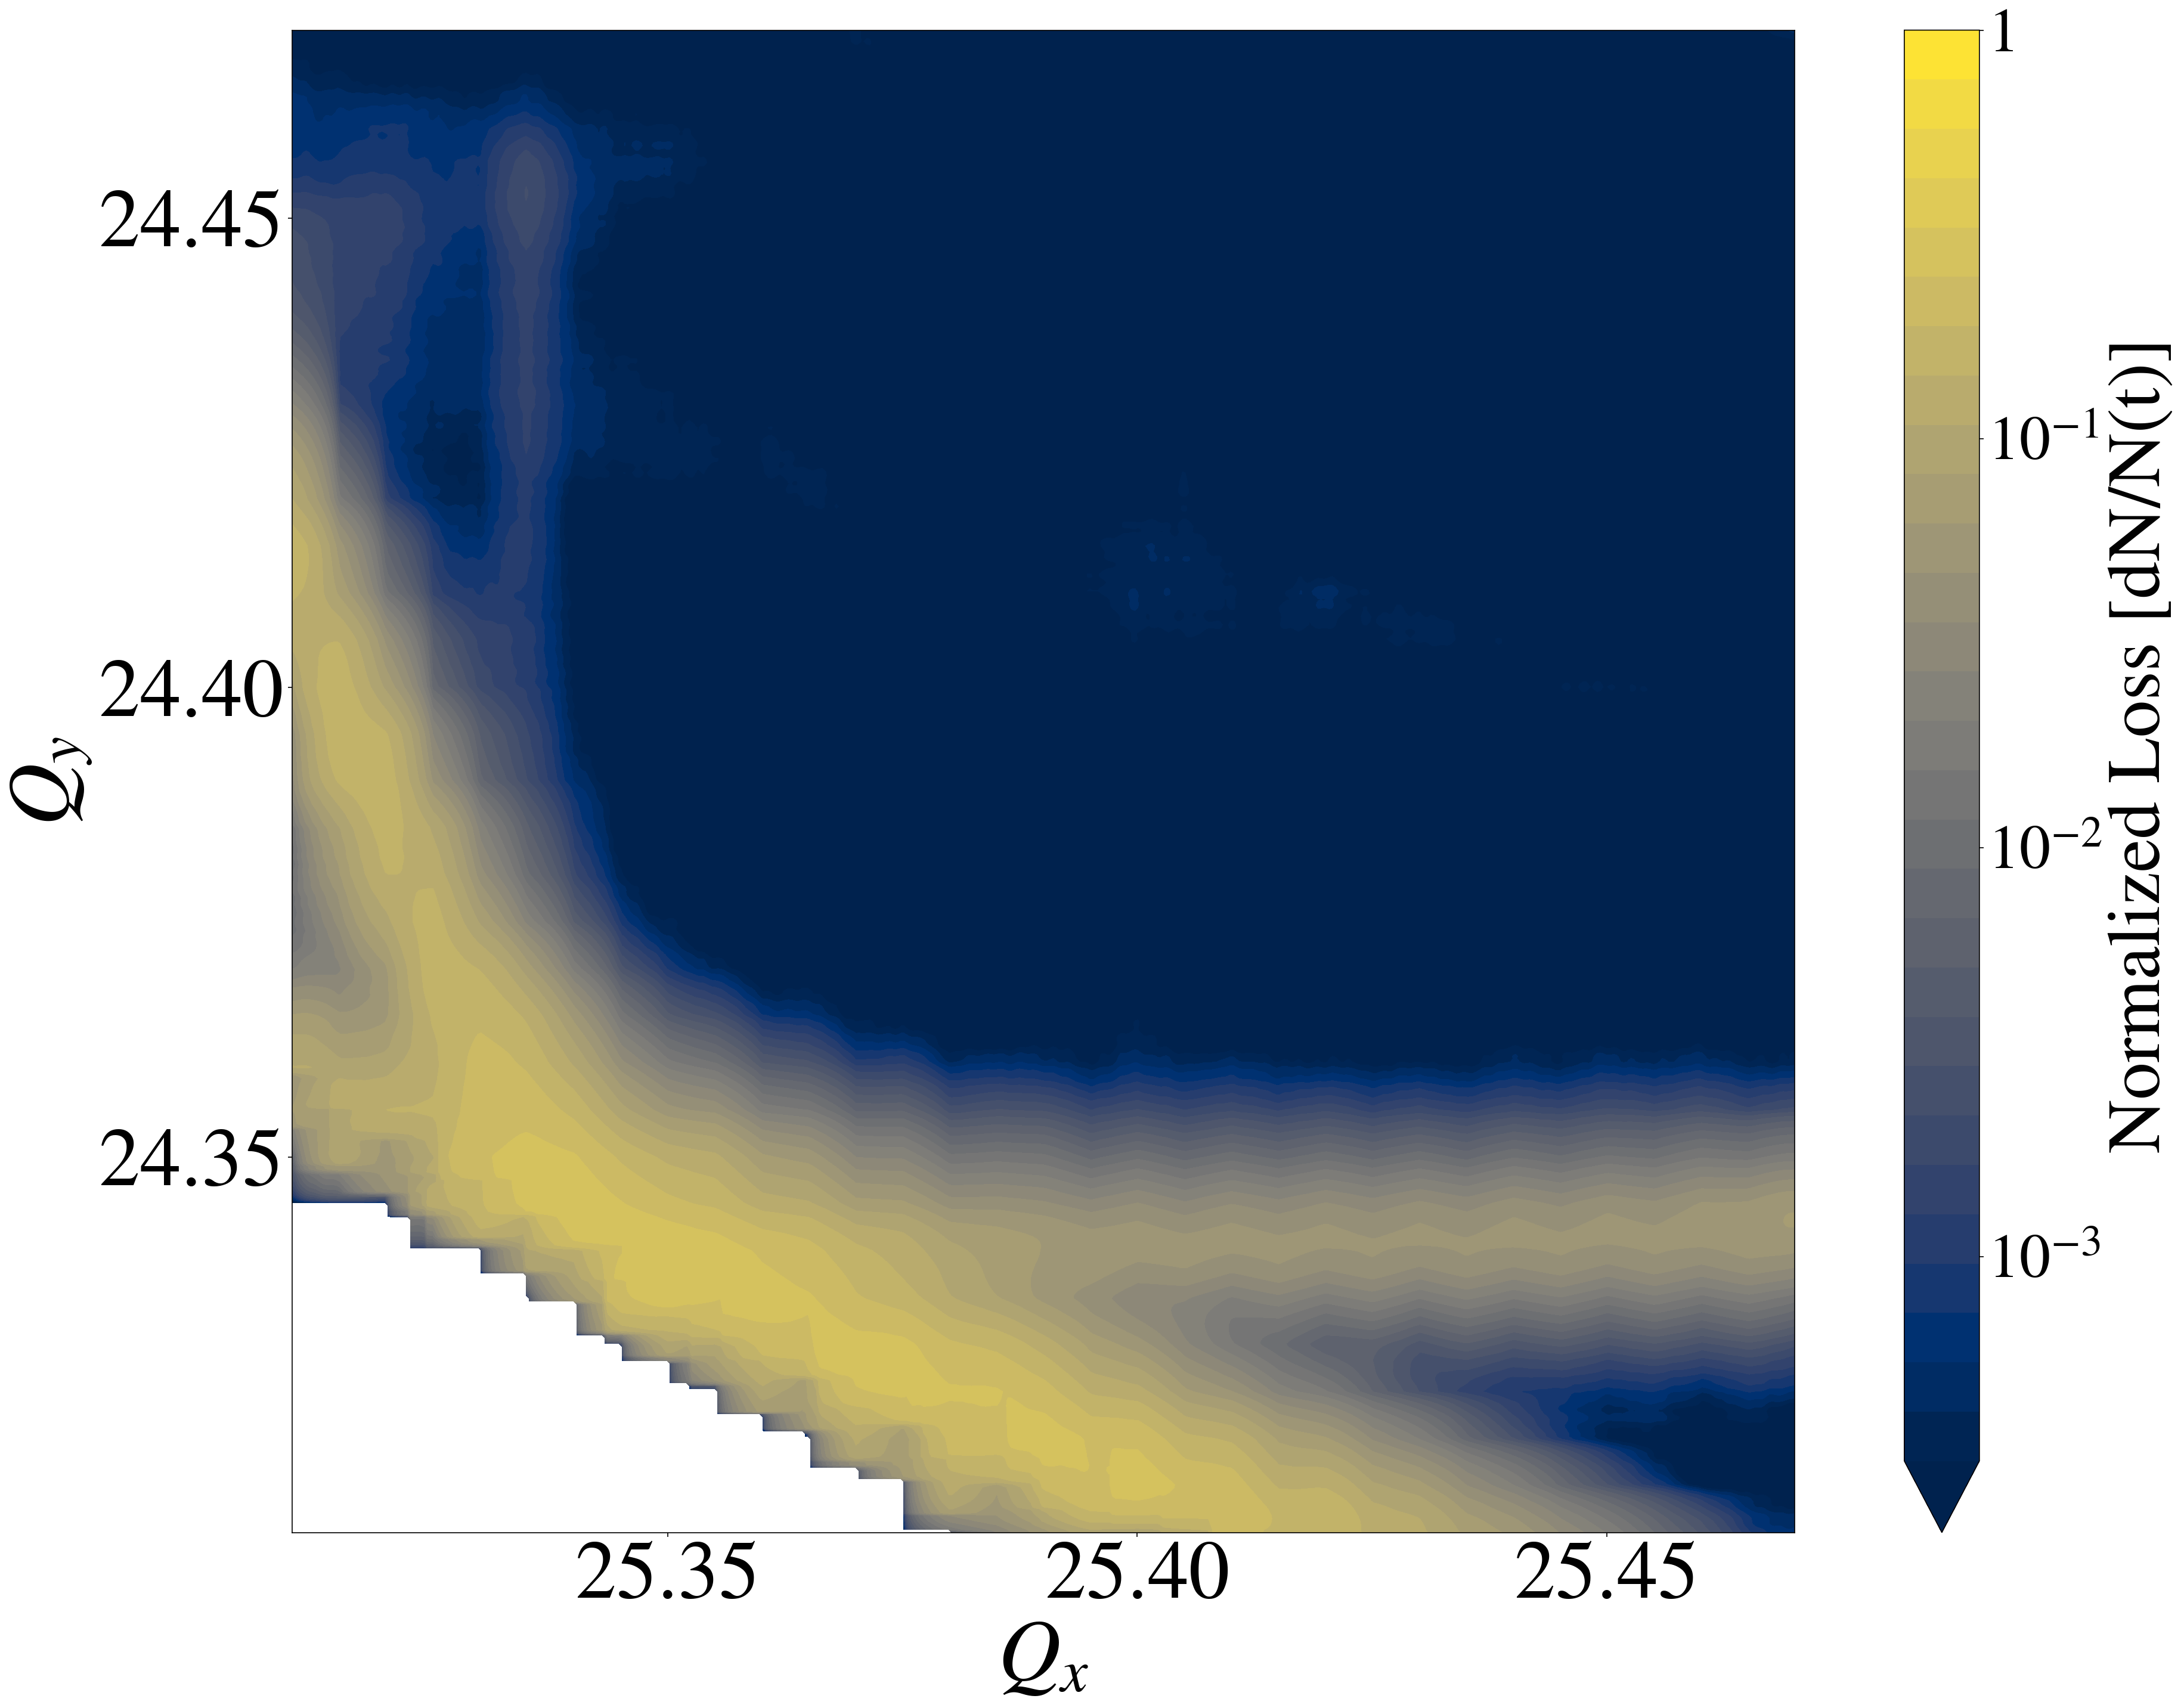
\includegraphics[width=0.98\linewidth]{chapter4/3qx.png}
      \caption{$3Q_x$ Compensation}
      \label{fig:sfig2}
    \end{subfigure}
    \hfill
    \begin{subfigure}{.49\textwidth}
      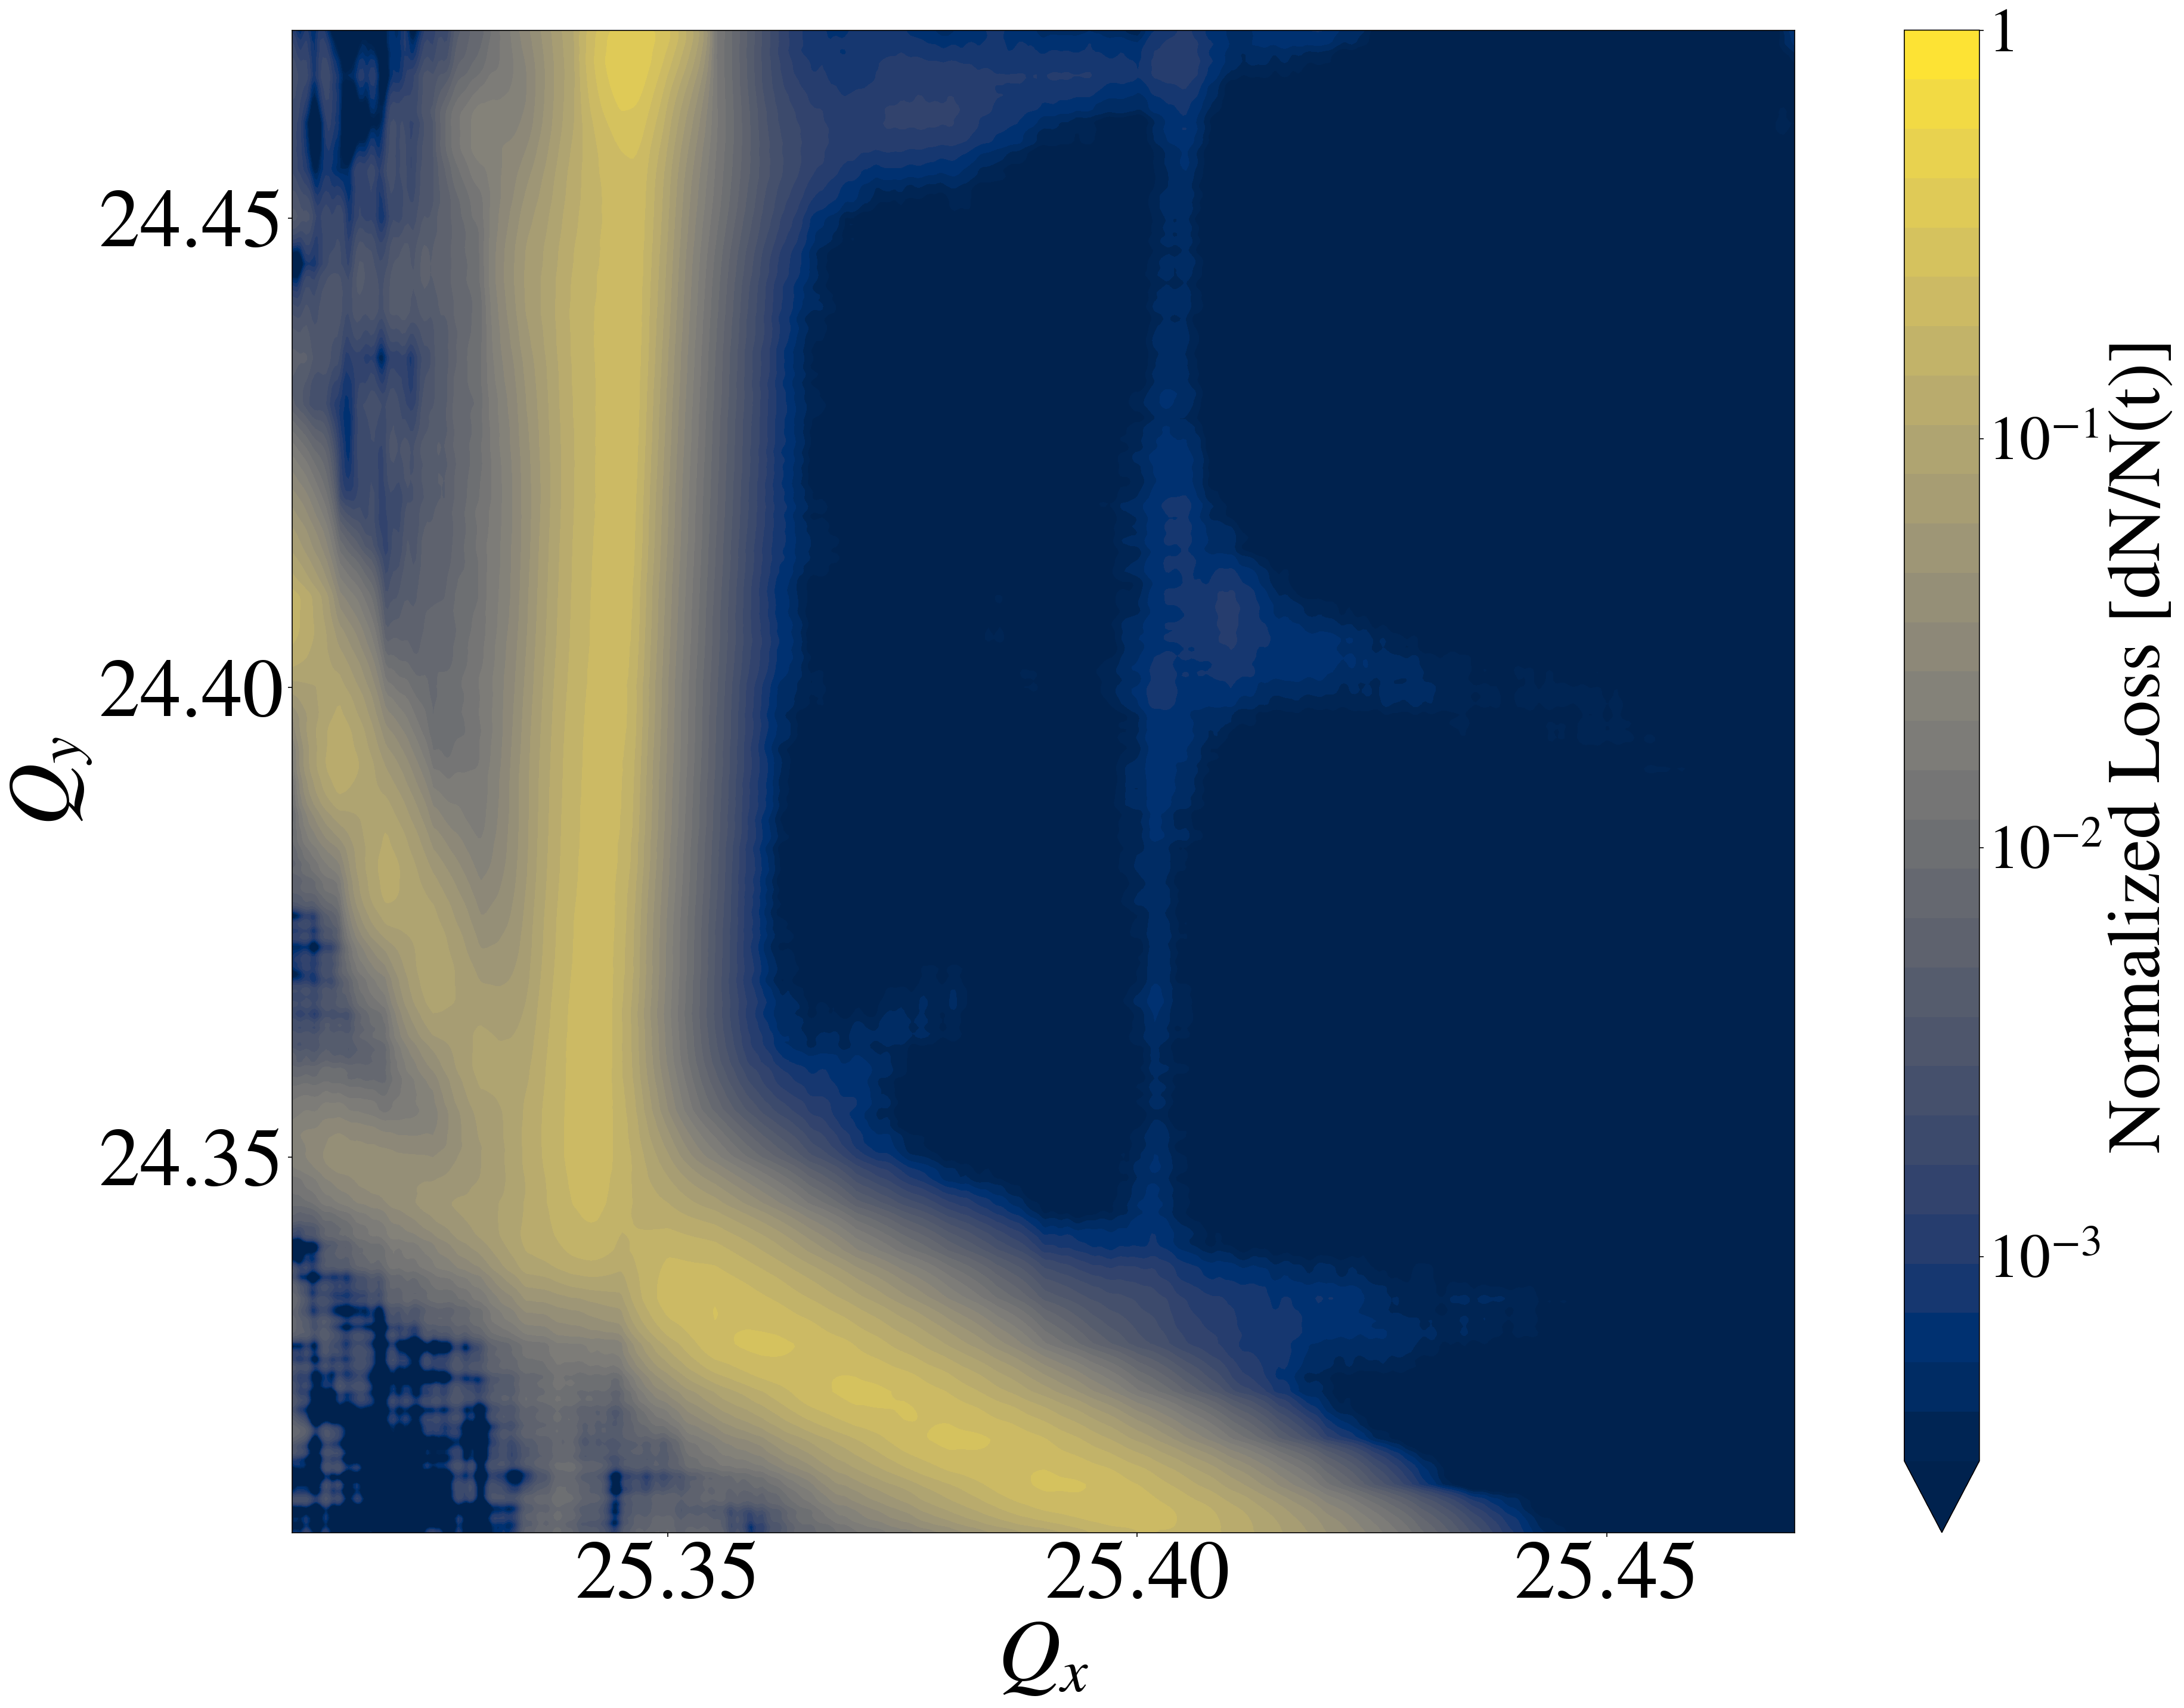
\includegraphics[width=0.98\linewidth]{chapter4/3qy.png}
      \caption{$3Q_y$ Compensation}
      \label{fig:sfig3}
    \end{subfigure}
    \hfill
    \begin{subfigure}{.49\textwidth}
      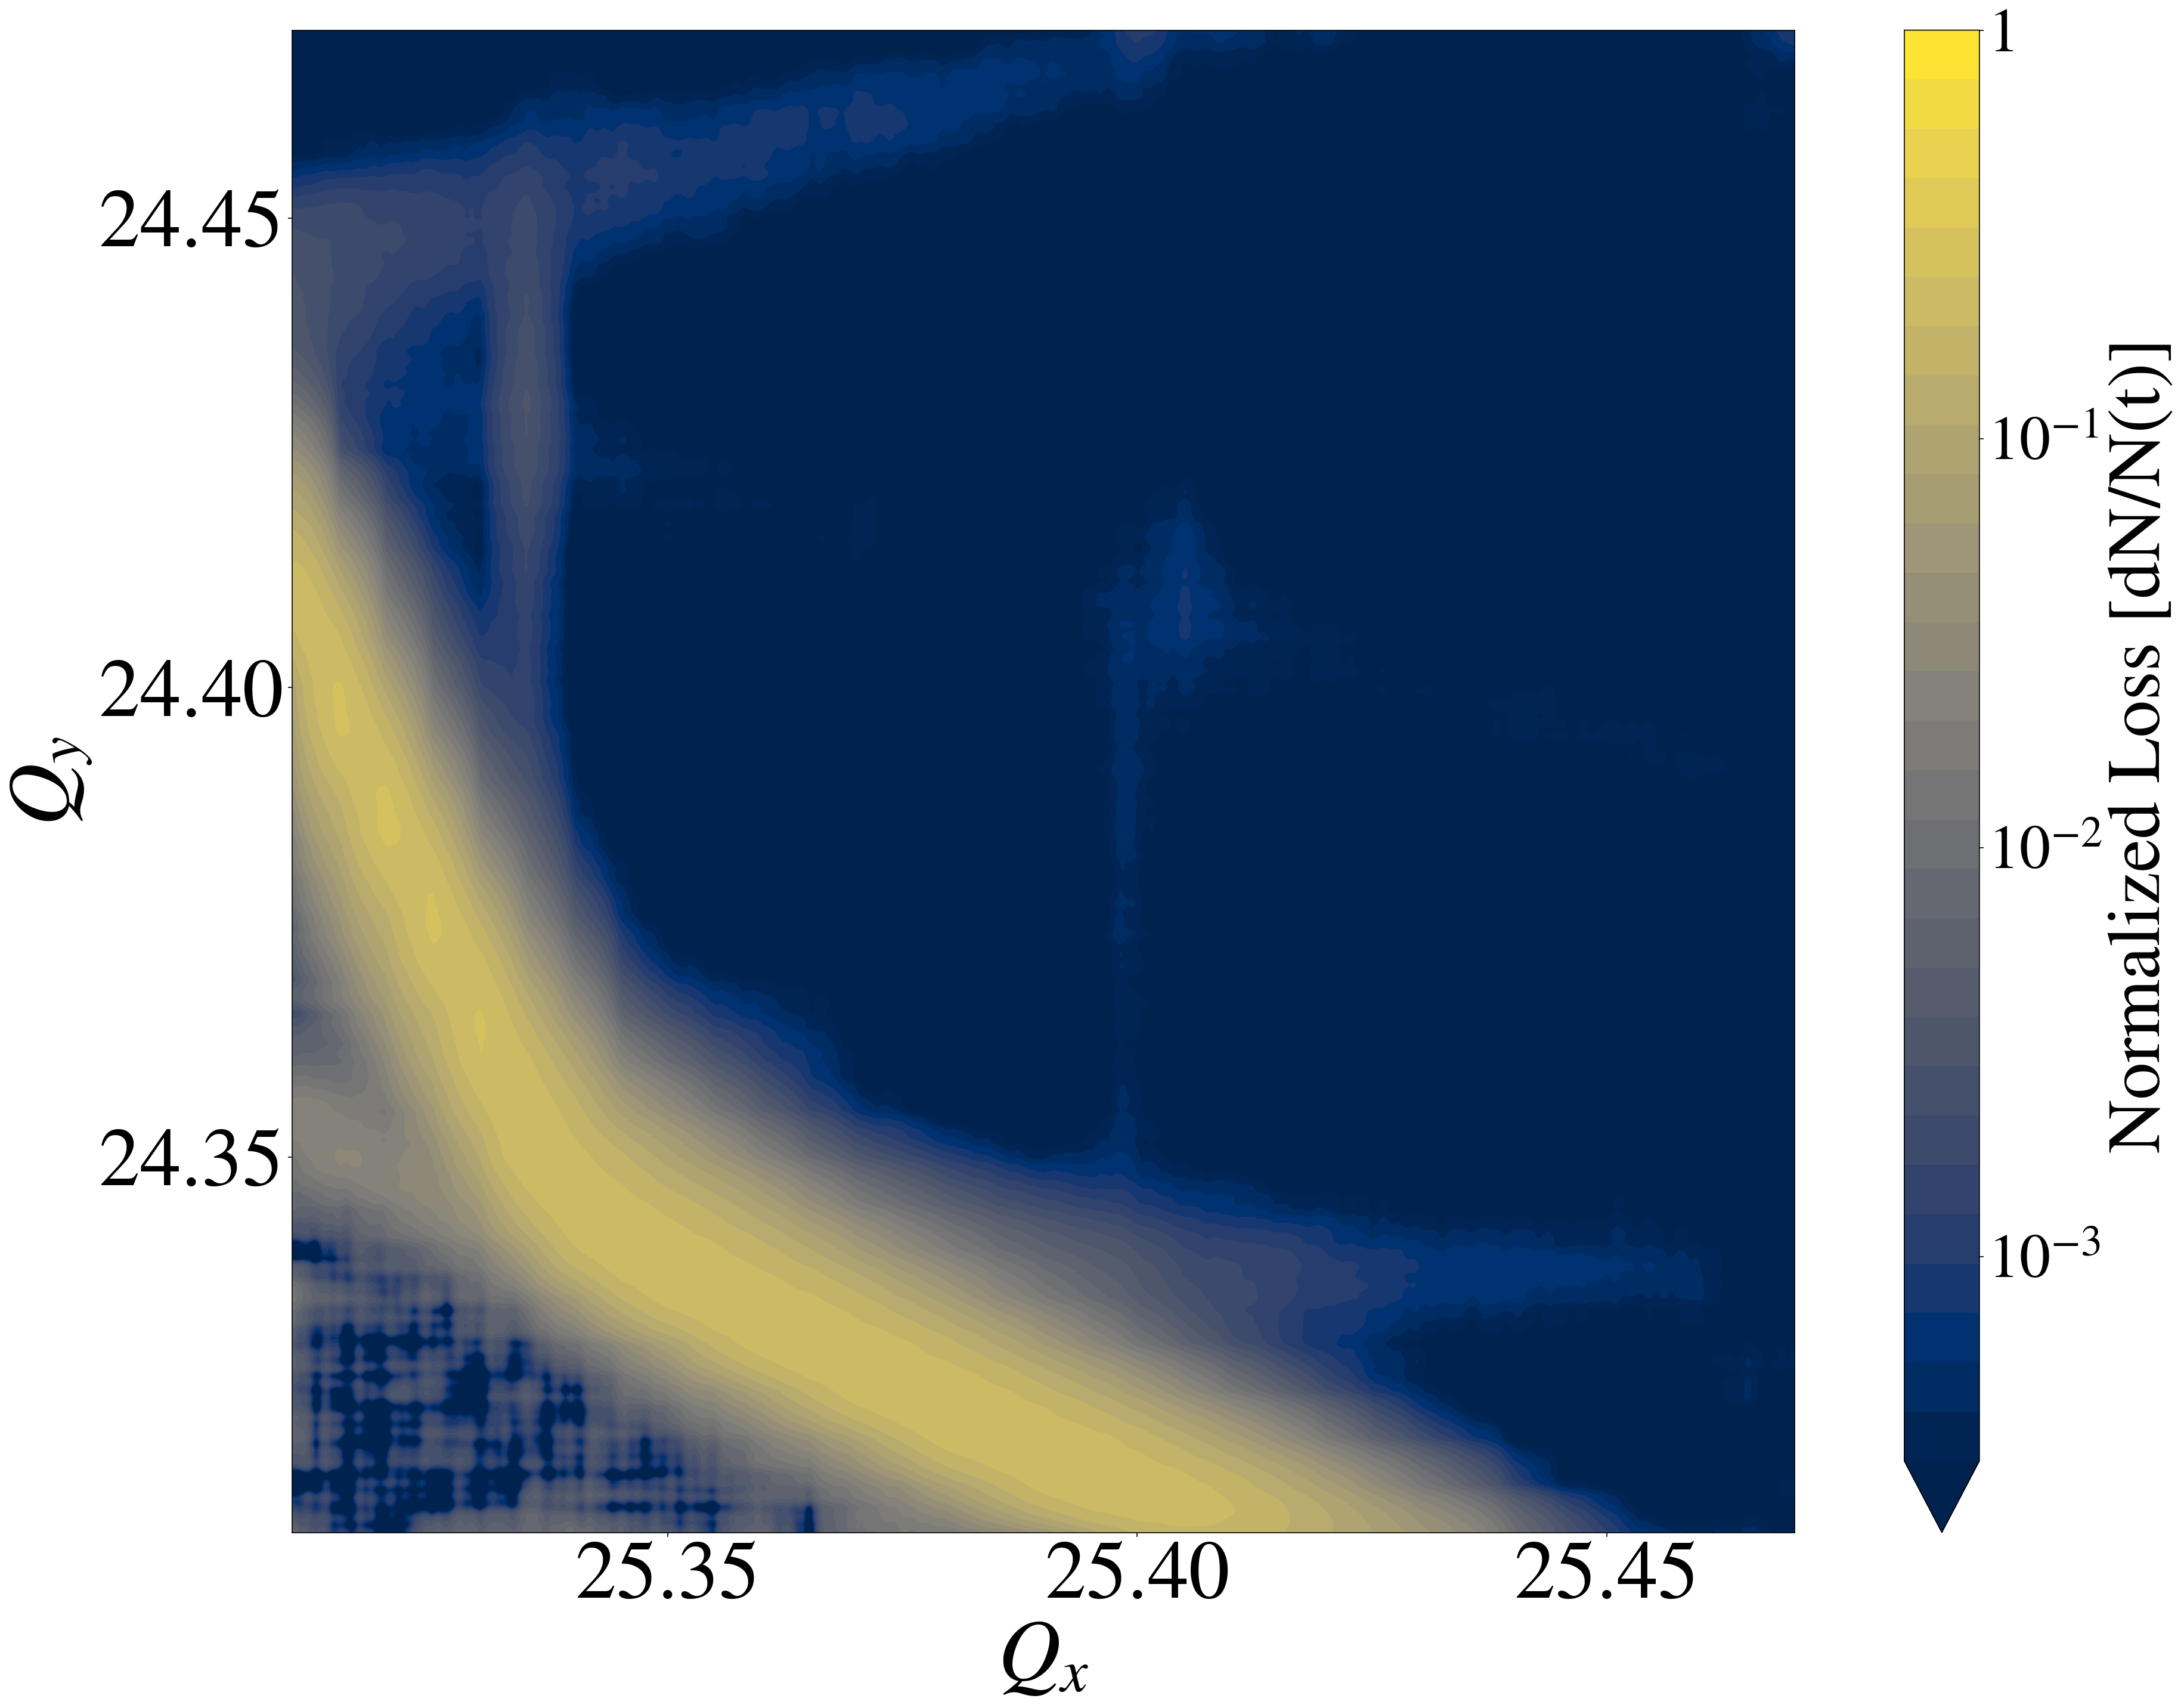
\includegraphics[width=0.98\linewidth]{chapter4/3qx_3qy.png}
      \caption{$3Q_x$ and $3Q_y$ Compensation}
      \label{fig:sfig4}
    \end{subfigure}%
    \hfill
    \begin{subfigure}{.49\textwidth}
      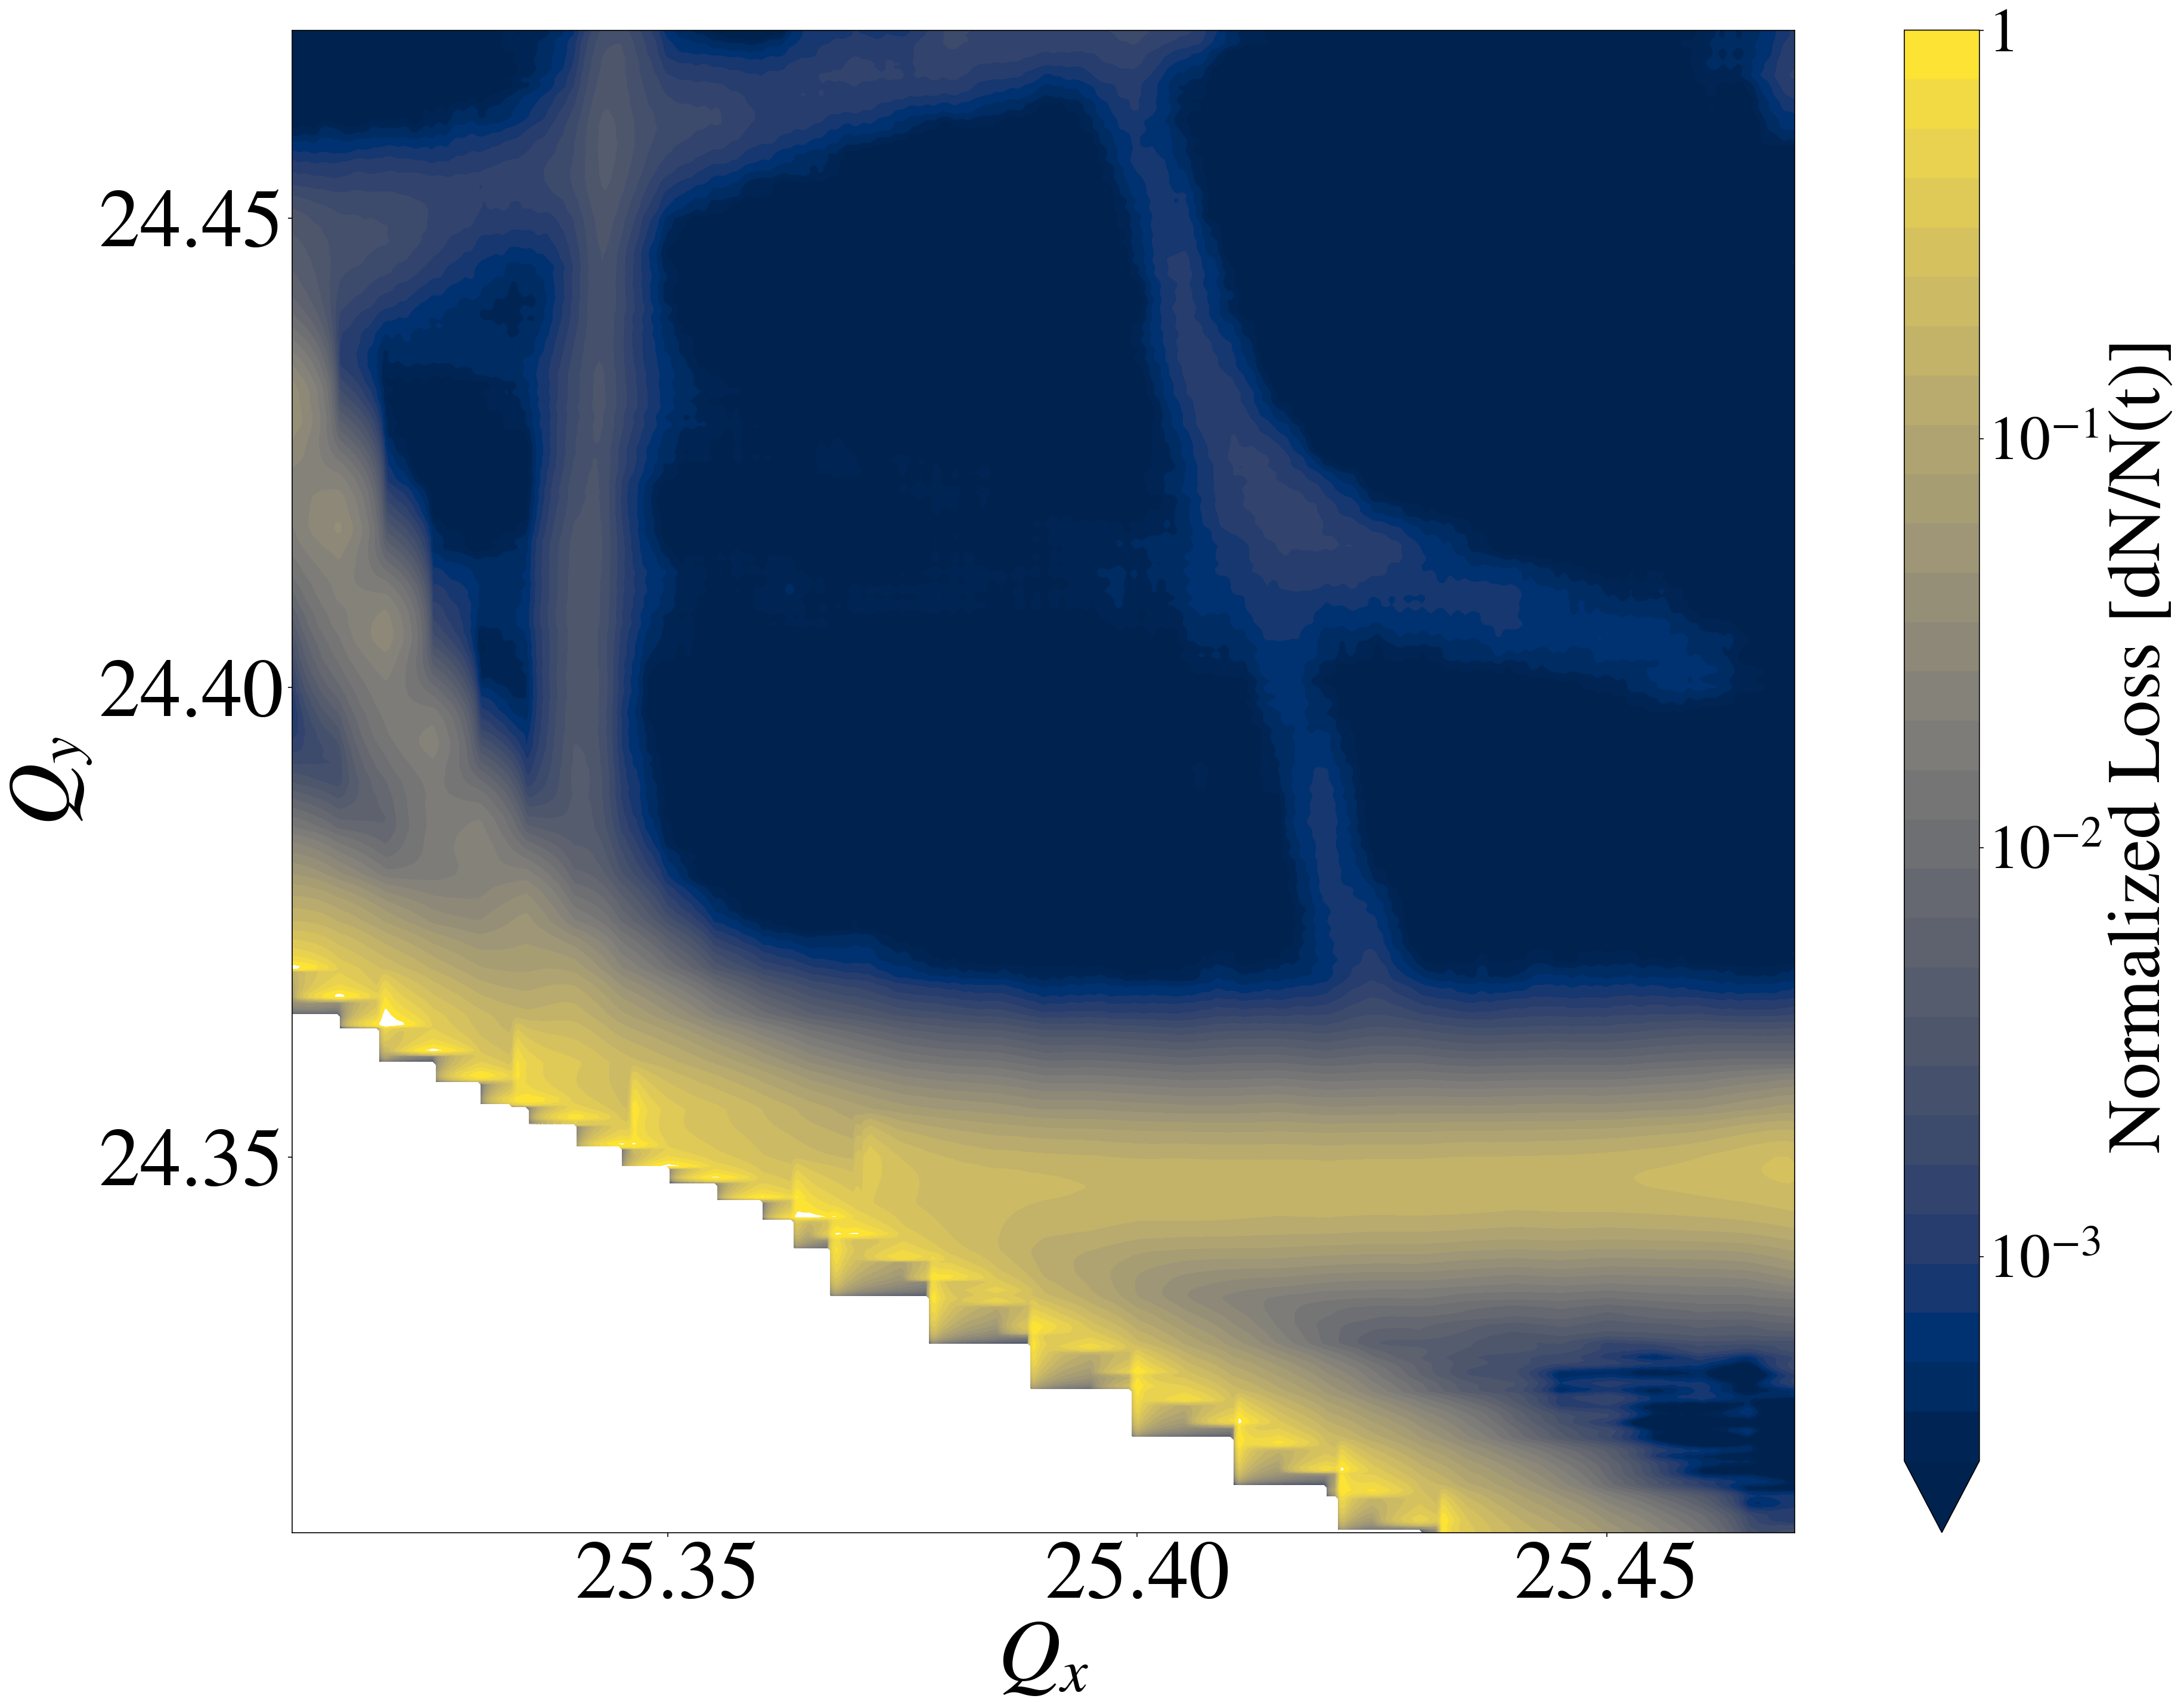
\includegraphics[width=0.98\linewidth]{chapter4/3qx_2qxqy.png}
      \caption{$3Q_x$ and $2Q_x+Q_y$ Compensation}
      \label{fig:sfig5}
    \end{subfigure}
    \hfill
    \begin{subfigure}{.49\textwidth}
      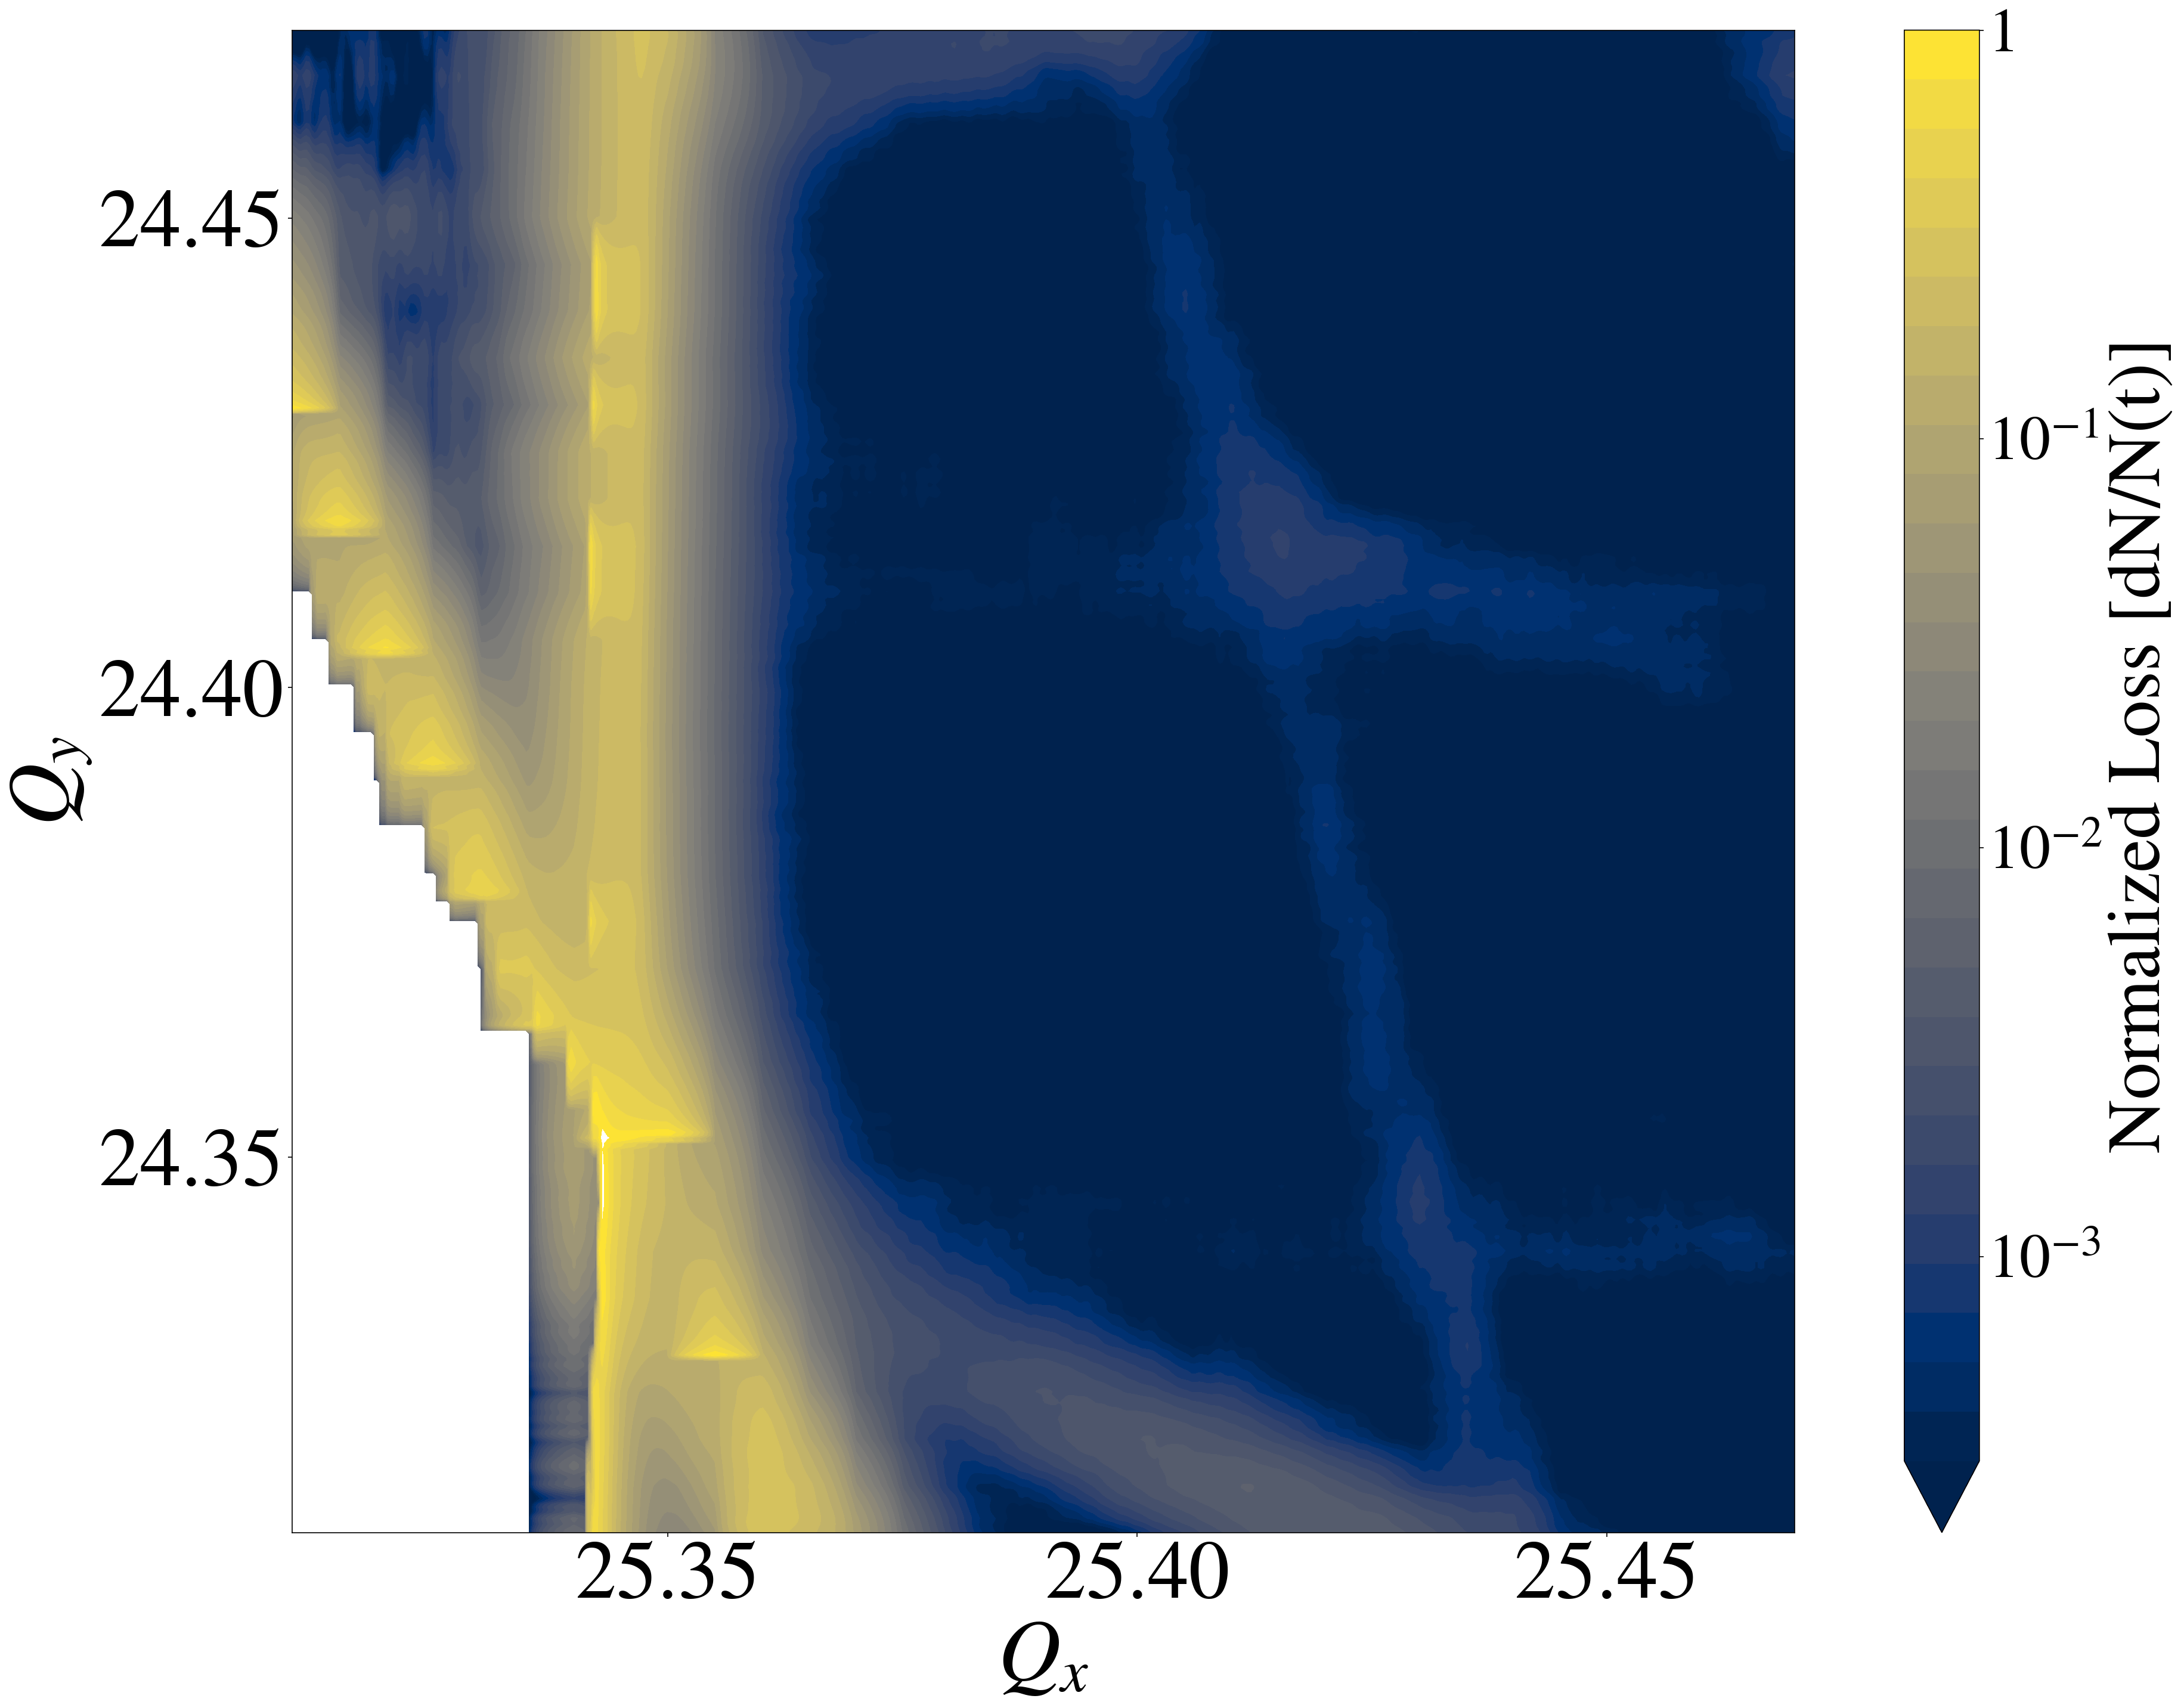
\includegraphics[width=0.98\linewidth]{chapter4/3qy_qx2qy.png}
      \caption{$3Q_y$ and $Q_x+2Q_y$ Compensation}
      \label{fig:sfig6}
    \end{subfigure}
    
    \caption{Dynamic loss maps for several configurations of compensation sextupoles}
    \label{fig:lossmaps}
    \end{figure} 
\newpage


\subsection{Static Tune Scans}

Another method for visualizing resonance compensation involves static tune scans. While the loss maps detailed earlier illustrate the dynamic crossing of resonance, an alternative method entails setting the tune to a specific value and assessing the beam survival ratio alongside the beam size over a defined time interval. The beam size is quantified using the Ion Profile Monitor System (IPM) within the ring, and the results are expressed in arbitrary units to indicate a relative effect.

\begin{figure}[H]
    \centering
    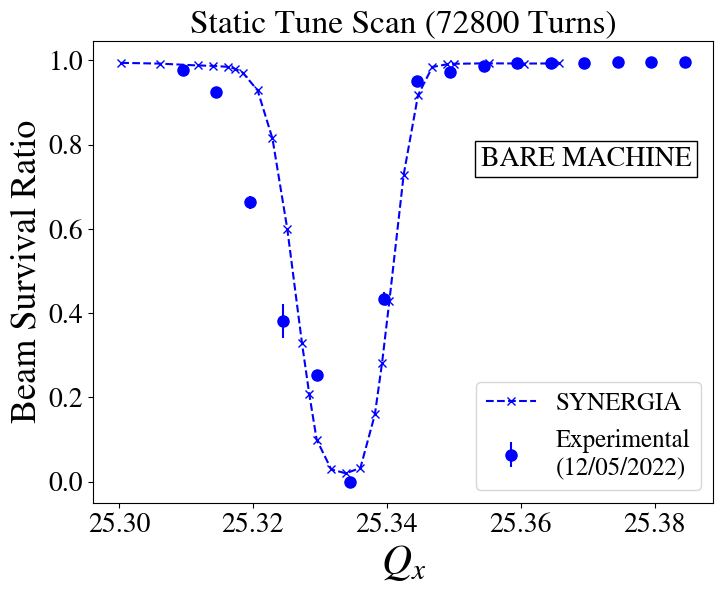
\includegraphics[width=\columnwidth]{chapter4/static2turns.png}
    \caption{Static tune scan for bare machine with comparisons between experimental data and SYNERGIA simulations.}
    \label{fig:static2}
\end{figure}

% \begin{figure}[H]
%     \centering
%     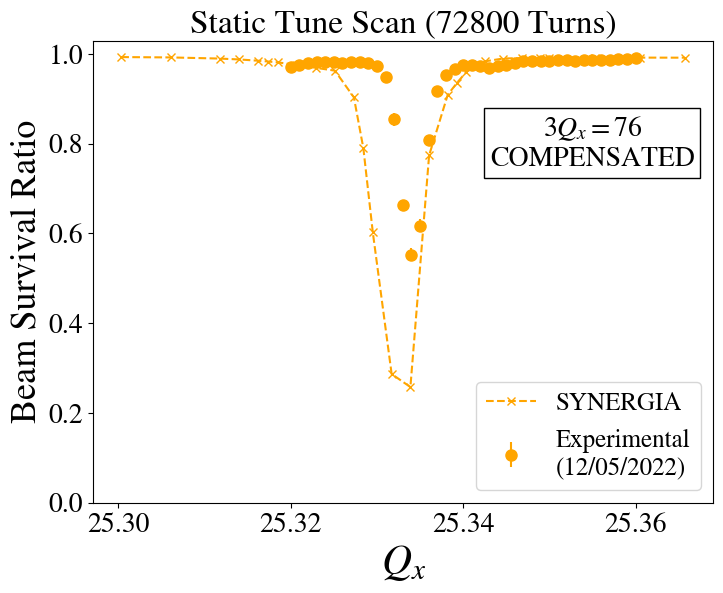
\includegraphics[width=\columnwidth]{chapter4/static2turns_comp.png}
%     \caption{Plot for static tune scan for machine with $3Q_x$ compensation including comparison between experimental data and SYNERGIA simulations.}
%     \label{fig:static2_comp}
% \end{figure}

\begin{figure}[H]
    \centering
    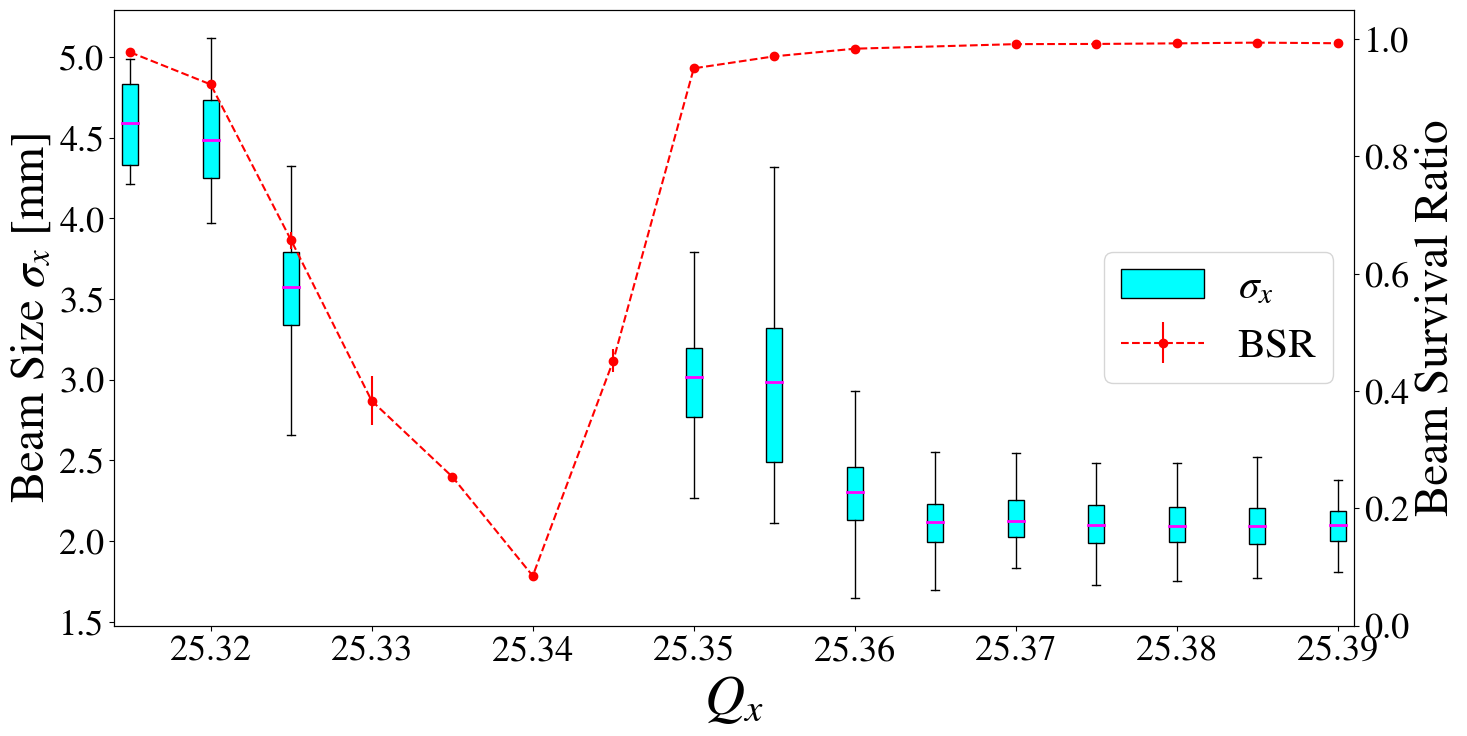
\includegraphics[width=\columnwidth]{chapter4/static2turns_ipm.png}
    \caption{Static tune scan with beam survival ratio and IPM data box plots for bare machine at 2 Booster Turns of equivalent intensity.}
    \label{fig:static2_ipm}
\end{figure}

\begin{figure}[H]
    \centering
    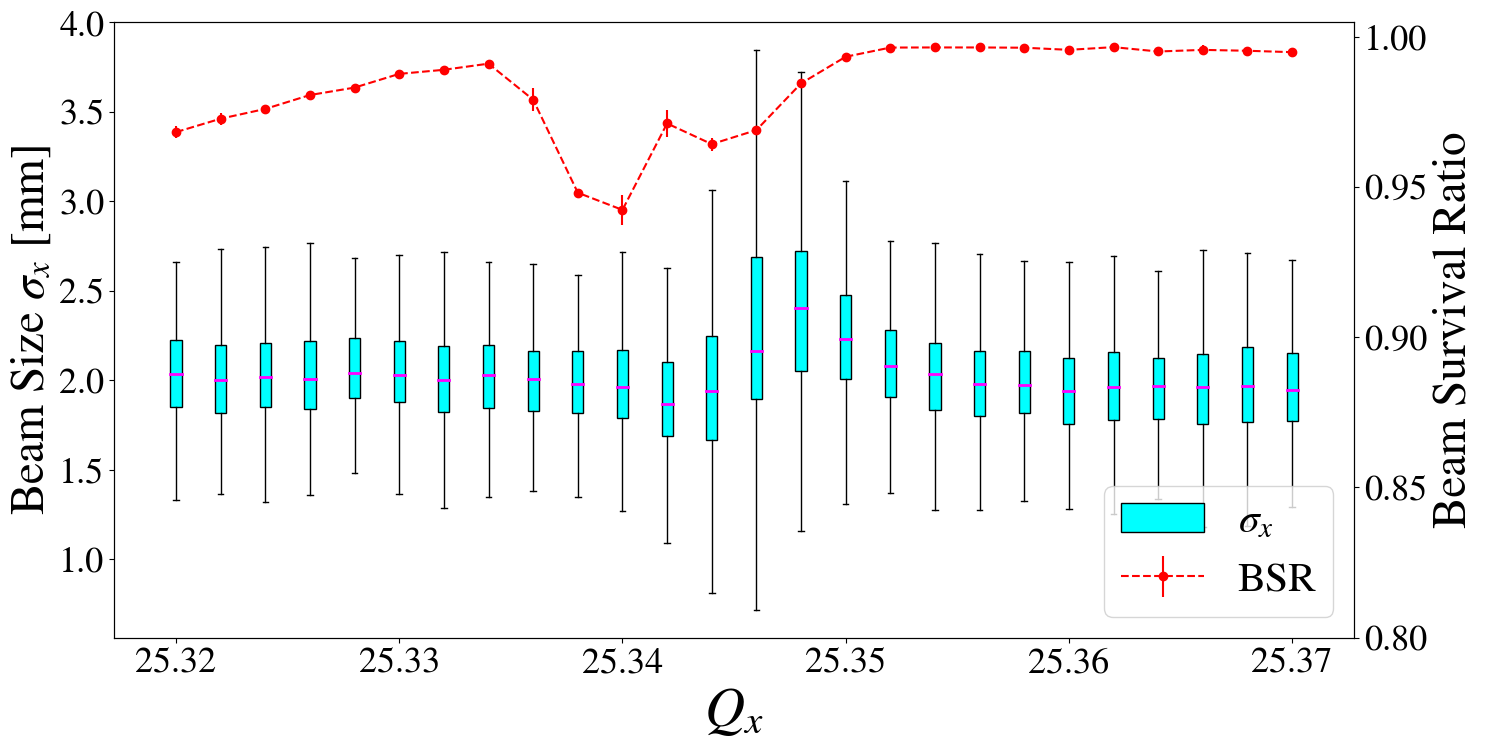
\includegraphics[width=\columnwidth]{chapter4/static2turns_comp_ipm_dampersOFF.png}
    \caption{Static tune scan with beam survival ratio and IPM data box plots for machine with $3Q_x$ compensation at 2 Booster Turns of equivalent intensity.}
    \label{fig:static2_ipm_comp}
\end{figure}

\section{Additional Sextupoles for Resonance Compensation}
\label{sec:addsexts}

\begin{equation}
    \begin{bmatrix}
        -|h_{3000}| \cos \psi_{3000} \\
        -|h_{3000}| \sin \psi_{3000} \\
        -|h_{1020}| \cos \psi_{1020} \\
        -|h_{1020}| \sin \psi_{1020} \\
        \end{bmatrix}_{(Bare)}
         =
        \boldsymbol{M}
        \begin{bmatrix}
        k_2^{(sc220)} \\
        k_2^{(sc222)}\\
        k_2^{(sc319)} \\
        k_2^{(sc321)}\\
        \end{bmatrix}
        \label{eq:systemk2s}        
\end{equation}

\begin{figure}[H]
    \centering
    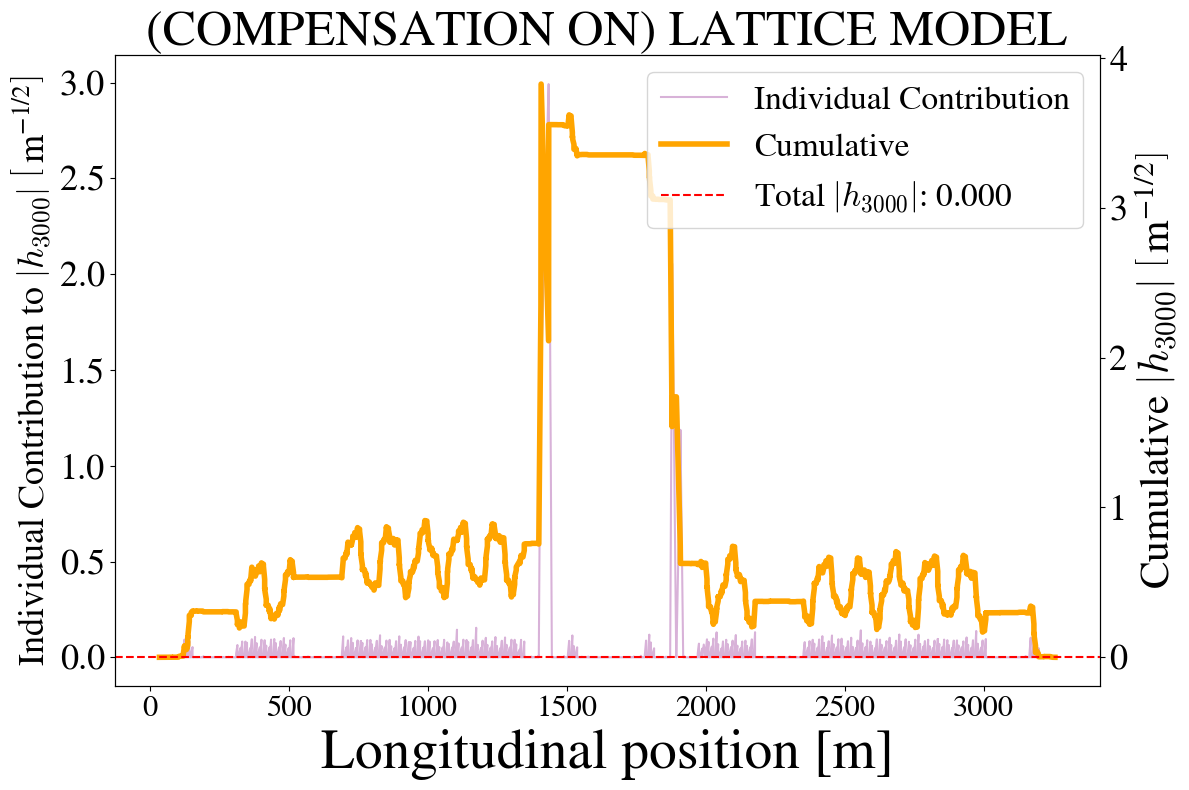
\includegraphics[width=\columnwidth]{chapter4/old_config_h3000.png}
    \caption{Distribution of the $h_{3000}$ term around the ring with individual contributions from each relevant element and the cumulative sum from an arbitrary starting point. This is with existing sextupoles powered at the correct currents to cancel out $h_{3000}$ and $h_{1020}$ simultaneously.}
    \label{fig:h3000oldconfig}
\end{figure}

\begin{figure}[H]
    \centering
    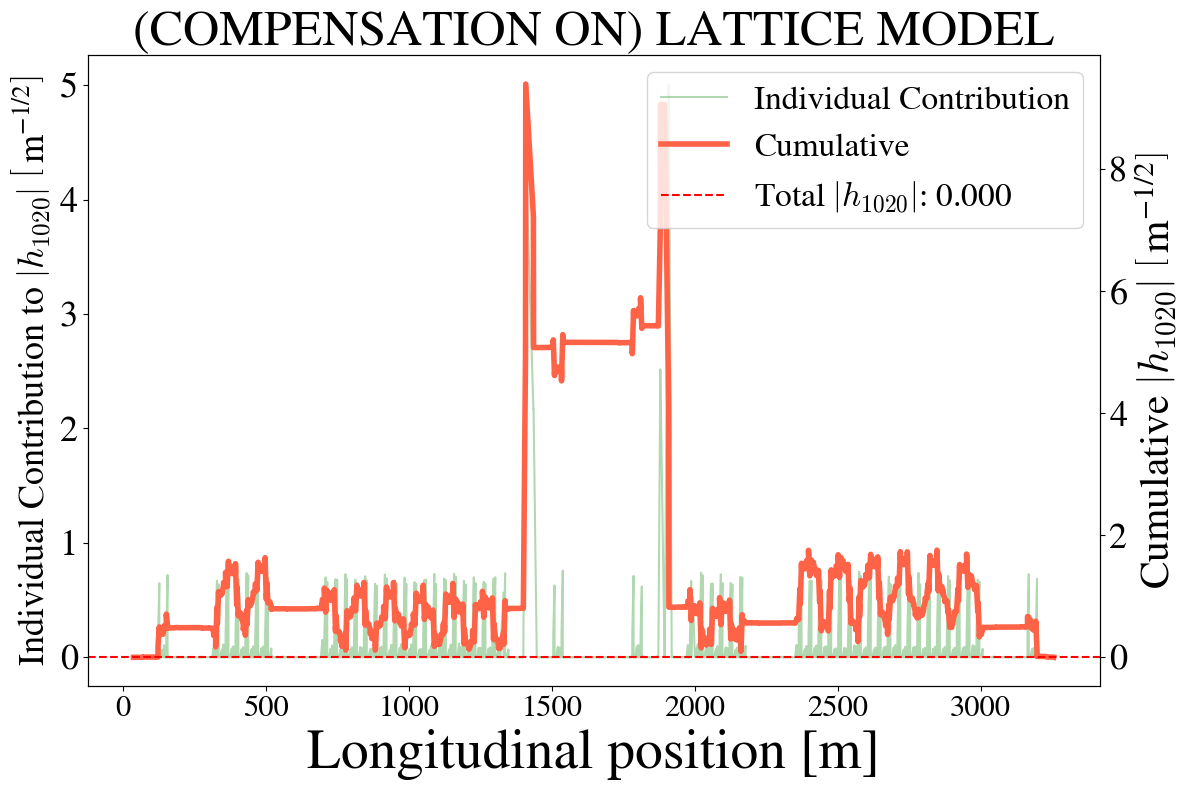
\includegraphics[width=\columnwidth]{chapter4/old_config_h1020.png}
    \caption{Distribution of the $h_{1020}$ term around the ring with individual contributions from each relevant element and the cumulative sum from an arbitrary starting point. This is with existing sextupoles powered at the correct currents to cancel out $h_{3000}$ and $h_{1020}$ simultaneously.}
    \label{fig:h1020oldconfig}
\end{figure}

\begin{equation}
    \begin{bmatrix}
        -|h_{3000}| \cos \psi_{3000} \\
        -|h_{3000}| \sin \psi_{3000} \\
        -|h_{1020}| \cos \psi_{1020} \\
        -|h_{1020}| \sin \psi_{1020} \\
        \end{bmatrix}_{(Bare)}
         =
        \boldsymbol{M}
        \begin{bmatrix}
        k_2^{(sc220)} \\
        k_2^{(sc222)}\\
        k_2^{(sc319)} \\
        k_2^{(sc321)}\\
        k_2^{(1)} \\
        k_2^{(2)}\\
        \end{bmatrix}
        \label{eq:systemadd}
\end{equation}

\begin{figure}[H]
    \centering
    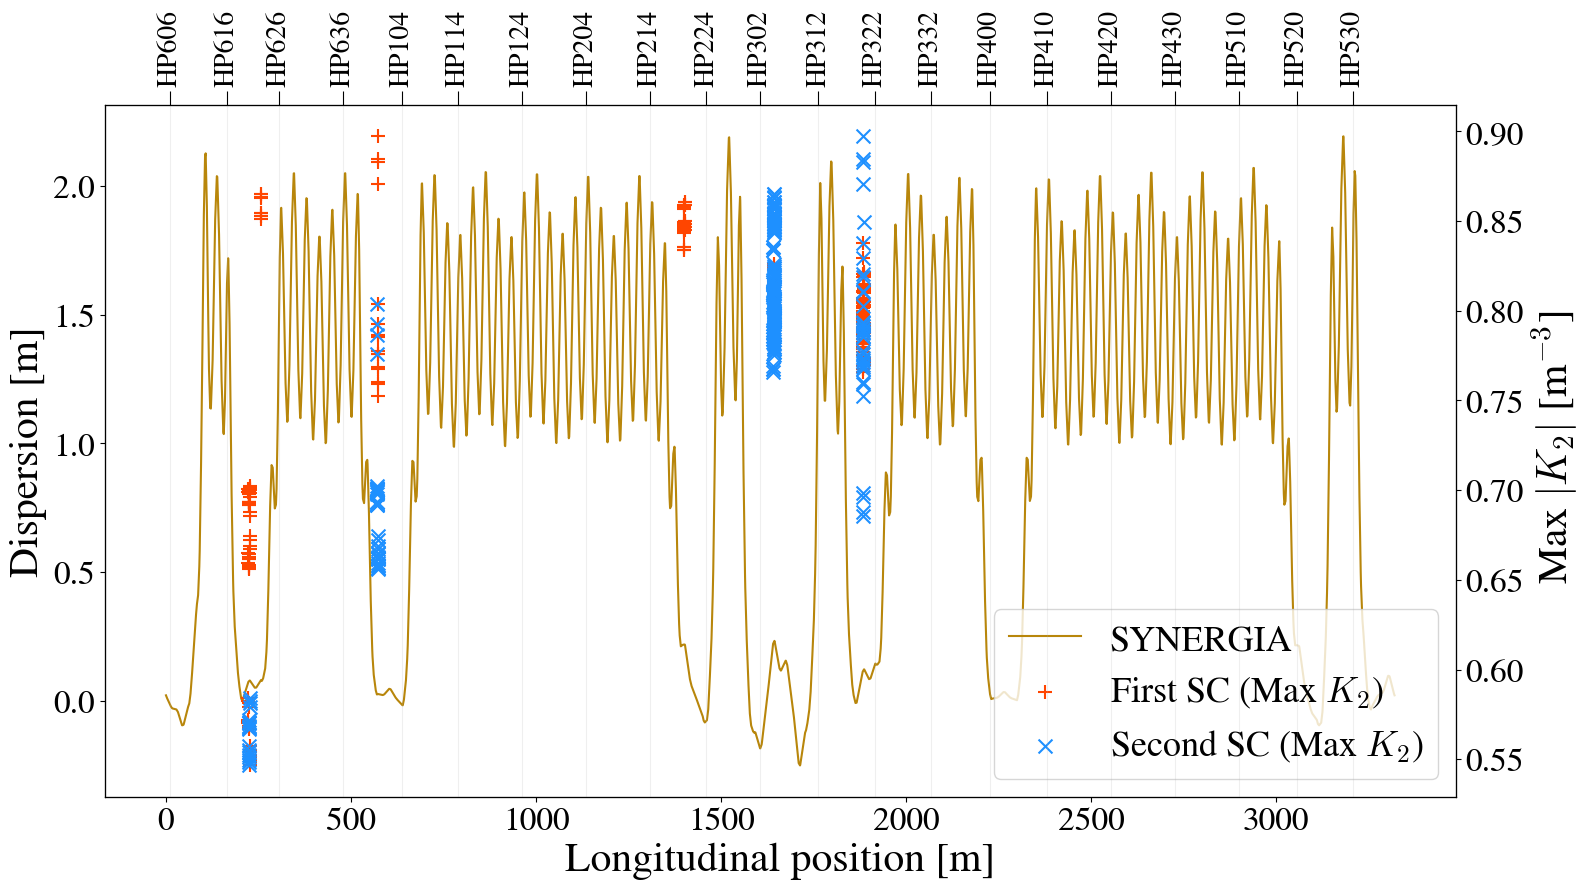
\includegraphics[width=\columnwidth]{chapter4/new_sexts_dx.png}
    \caption{Dispersion function of the Recycler Ring with possible new locations to introduce a pair of sextupole magnets that cancel out $h_{3000}$ and $h_{1020}$ simultaneously. The right y-axis shows the maximum compensation current needed with these new candidates.}
    \label{fig:dxnewsexts}
\end{figure}

\begin{figure}[H]
    \centering
    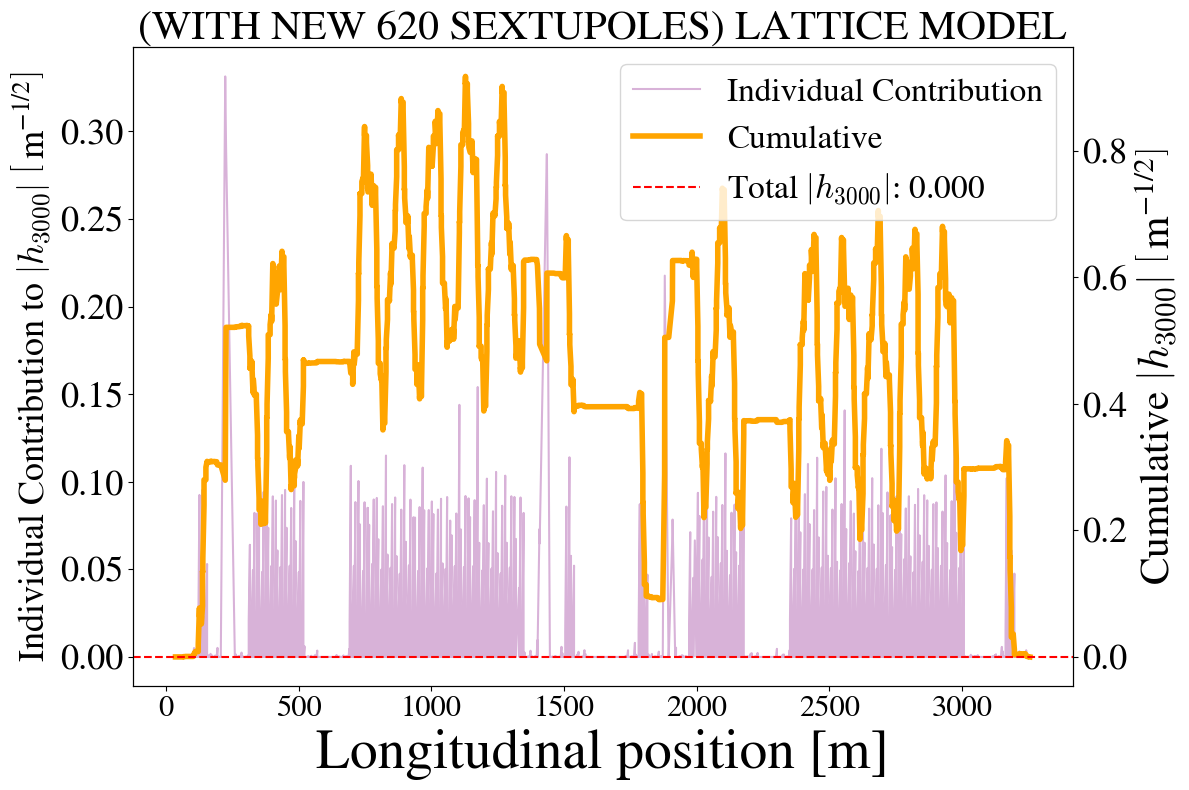
\includegraphics[width=\columnwidth]{chapter4/new_sexts_h3000.png}
    \caption{Distribution of the $h_{3000}$ term around the ring with individual contributions from each relevant element and the cumulative sum from an arbitrary starting point. This is with the new 620 sextupoles powered at the correct currents to cancel out $h_{3000}$ and $h_{1020}$ simultaneously.}
    \label{fig:h3000newsexts}
\end{figure}

\begin{figure}[H]
    \centering
    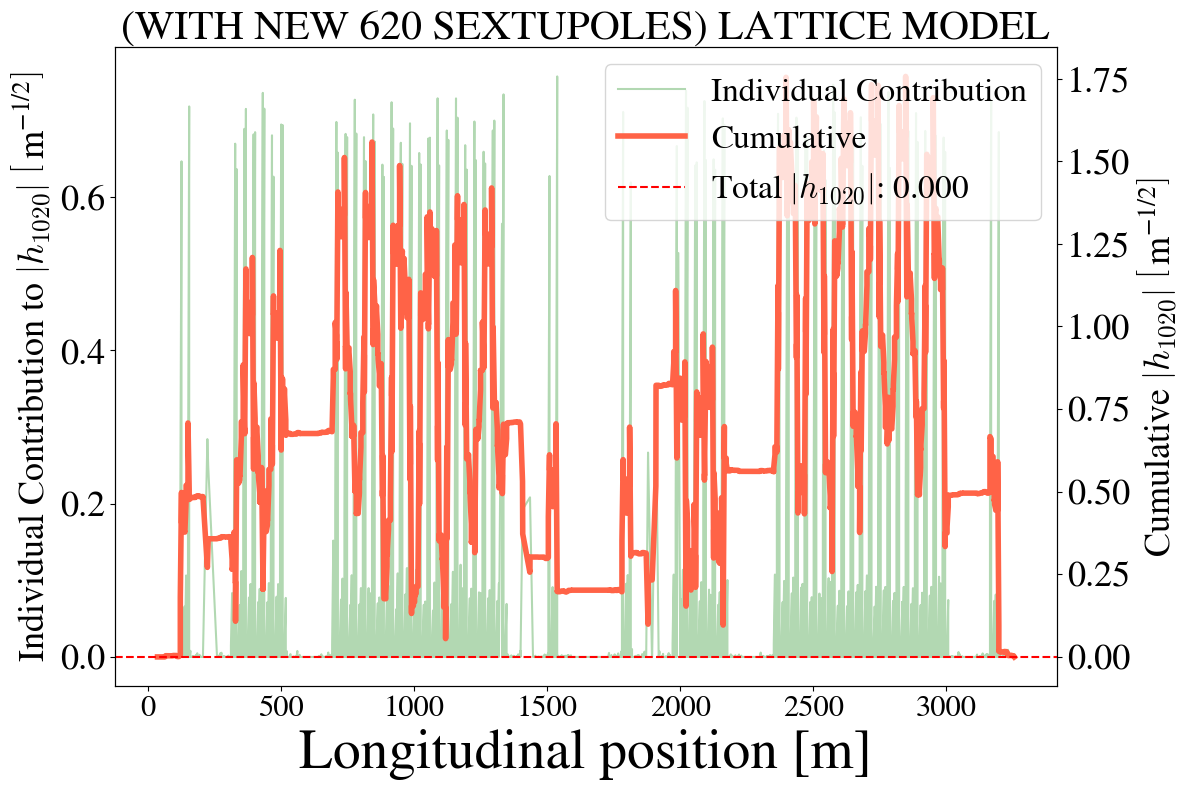
\includegraphics[width=\columnwidth]{chapter4/new_sexts_h1020.png}
    \caption{Distribution of the $h_{1020}$ term around the ring with individual contributions from each relevant element and the cumulative sum from an arbitrary starting point. This is with the new 620 sextupoles powered at the correct currents to cancel out $h_{3000}$ and $h_{1020}$ simultaneously.}
    \label{fig:h1020newsexts}
\end{figure}
